\PassOptionsToPackage{unicode=true}{hyperref} % options for packages loaded elsewhere
\PassOptionsToPackage{hyphens}{url}
%
\documentclass[11pt,]{article}
\usepackage{lmodern}
\usepackage{amssymb,amsmath}
\usepackage{ifxetex,ifluatex}
\usepackage{fixltx2e} % provides \textsubscript
\ifnum 0\ifxetex 1\fi\ifluatex 1\fi=0 % if pdftex
  \usepackage[T1]{fontenc}
  \usepackage[utf8]{inputenc}
  \usepackage{textcomp} % provides euro and other symbols
\else % if luatex or xelatex
  \usepackage{unicode-math}
  \defaultfontfeatures{Ligatures=TeX,Scale=MatchLowercase}
\fi
% use upquote if available, for straight quotes in verbatim environments
\IfFileExists{upquote.sty}{\usepackage{upquote}}{}
% use microtype if available
\IfFileExists{microtype.sty}{%
\usepackage[]{microtype}
\UseMicrotypeSet[protrusion]{basicmath} % disable protrusion for tt fonts
}{}
\IfFileExists{parskip.sty}{%
\usepackage{parskip}
}{% else
\setlength{\parindent}{0pt}
\setlength{\parskip}{6pt plus 2pt minus 1pt}
}
\usepackage{hyperref}
\hypersetup{
            pdfauthor={Benoît Verhaeghe},
            pdfborder={0 0 0},
            breaklinks=true}
\urlstyle{same}  % don't use monospace font for urls
\usepackage[margin=2cm]{geometry}
\usepackage{graphicx,grffile}
\makeatletter
\def\maxwidth{\ifdim\Gin@nat@width>\linewidth\linewidth\else\Gin@nat@width\fi}
\def\maxheight{\ifdim\Gin@nat@height>\textheight\textheight\else\Gin@nat@height\fi}
\makeatother
% Scale images if necessary, so that they will not overflow the page
% margins by default, and it is still possible to overwrite the defaults
% using explicit options in \includegraphics[width, height, ...]{}
\setkeys{Gin}{width=\maxwidth,height=\maxheight,keepaspectratio}
\setlength{\emergencystretch}{3em}  % prevent overfull lines
\providecommand{\tightlist}{%
  \setlength{\itemsep}{0pt}\setlength{\parskip}{0pt}}
\setcounter{secnumdepth}{5}
% Redefines (sub)paragraphs to behave more like sections
\ifx\paragraph\undefined\else
\let\oldparagraph\paragraph
\renewcommand{\paragraph}[1]{\oldparagraph{#1}\mbox{}}
\fi
\ifx\subparagraph\undefined\else
\let\oldsubparagraph\subparagraph
\renewcommand{\subparagraph}[1]{\oldsubparagraph{#1}\mbox{}}
\fi

% set default figure placement to htbp
\makeatletter
\def\fps@figure{htbp}
\makeatother

\usepackage{hyperref}
\usepackage{graphicx}
\usepackage[french]{babel}
\usepackage{pdfpages}

\author{Benoît Verhaeghe}
\date{}

\begin{document}

\renewcommand{\tablename}{Tableau}
\begin{titlepage}


\includegraphics[width=3.7cm, height=2cm]{logo/inria.png}
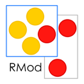
\includegraphics[width=2cm, height=2cm]{logo/rmod.png}

\includegraphics[width=4.5cm, height=2cm]{logo/polytech.jpg}
\hfill

\includegraphics[width=4cm, height=2cm]{logo/BL_logo.jpg}
\begin{center}

\vspace*{2.5cm}

\Large Benoît Verhaeghe

\vspace{1.5cm}

\Huge Migration d'application GWT vers Angular

\vspace{2.5cm}

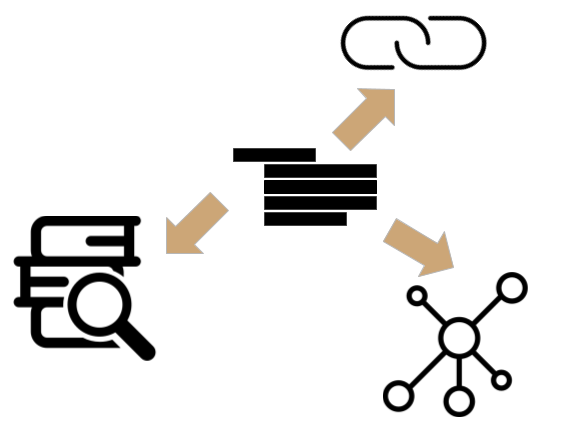
\includegraphics[width=13cm, height=7cm]{figures/intro.png}

\vfill

\normalsize Tuteurs entreprise : M. Deruelle, M. Seriai \\
Tuteur école : Mme Etien \\
Responsables Inria : Mme Etien, M. Anquetil

\vspace{0.8cm}

\normalsize Berger-Levrault \\ Inria Lille Nord Europe - RMod \\ août 2018

\end{center}
\end{titlepage}

\tableofcontents

\newpage

\hypertarget{contexte}{%
\section{Contexte}\label{contexte}}

\hypertarget{contexte-guxe9nuxe9ral}{%
\subsection{Contexte général}\label{contexte-guxe9nuxe9ral}}

Mon stage en entreprise est un travail qui s'inscrit dans le contexte
d'une collaboration entre l'équipe RMoD d'Inria Lille Nord Europe et
Berger-Levrault.

Berger-Levrault invente et développe des solutions pour les
administrations et les collectivités locales, pour les établissements
d'éducation et de santé publics comme privés, les universités et les
entreprises. L'entreprise est implantée en France, au Canada et en
Espagne.

J'ai travaillé dans l'équipe recherche et développement de
Berger-Levrault à Montpellier. Mes superviseurs entreprises étaient M.
Laurent Deruelle et M. Abderrahmane Seriai. Ma tutrice école était Mme
Anne Etien. J'ai, dans le cadre de la collaboration entre
Berger-Levrault et l'Inria Lille Nord Europe, travaillé aussi avec M.
Nicolas Anquetil.

Ce travail est la suite du travail préliminaire que j'ai mené pendant
mon Projet de Fin d'Étude à Polytech Lille.

\hypertarget{probluxe9matique}{%
\subsection{Problématique}\label{probluxe9matique}}

Berger-Levrault possède des applications client/serveur qu'elle souhaite
rajeunir. En particulier, le front-end est développé en GWT et doit
migrer vers Angular 6. Le back-end est une application monolithique et
doit évoluer vers une architecture de services Web. Le changement de
framework\footnote{Framework: ensemble cohérent de composants logiciels
  structurels, qui sert à créer les fondations ainsi que les grandes
  lignes de tout ou d'une partie d'un logiciel (architecture).}
graphique est imposé par l'arrêt du développement de GWT par Google et
le problème de compatibilité arrière entre Angular 6 et Angular 1
(AngularJS). Le passage à une architecture à services est aussi souhaité
pour améliorer l'offre commerciale et la rendre plus flexible.

Mon travail durant ce stage ne traite que de la migration des
applications front-end.

\hypertarget{description-du-probluxe8me}{%
\subsection{Description du problème}\label{description-du-probluxe8me}}

Les applications front-end de Berger-Levrault sont développées en Java
en utilisant le framework GWT de Google. Dans l'optique d'homogénéiser
le visuel de leurs applications, Berger-Levrault a étendu ce framework.
Cette extension s'appelle \textbf{BLCore}. La Figure
\ref{architectureBL} représente les différentes couches de framework
utilisé par une application de Berger-Levrault. Les applications
utilisent et/ou étendent \textbf{BLCore}, qui lui même utilise et/ou
étend \textbf{GWT}. On retrouve aussi des applications, qui ne
respectent pas la convention décidé par les équipes de Berger-Levrault,
ayant un lien direct avec le framework \textbf{GWT}.

\hypertarget{architectureBL}{%
\begin{figure}
\centering
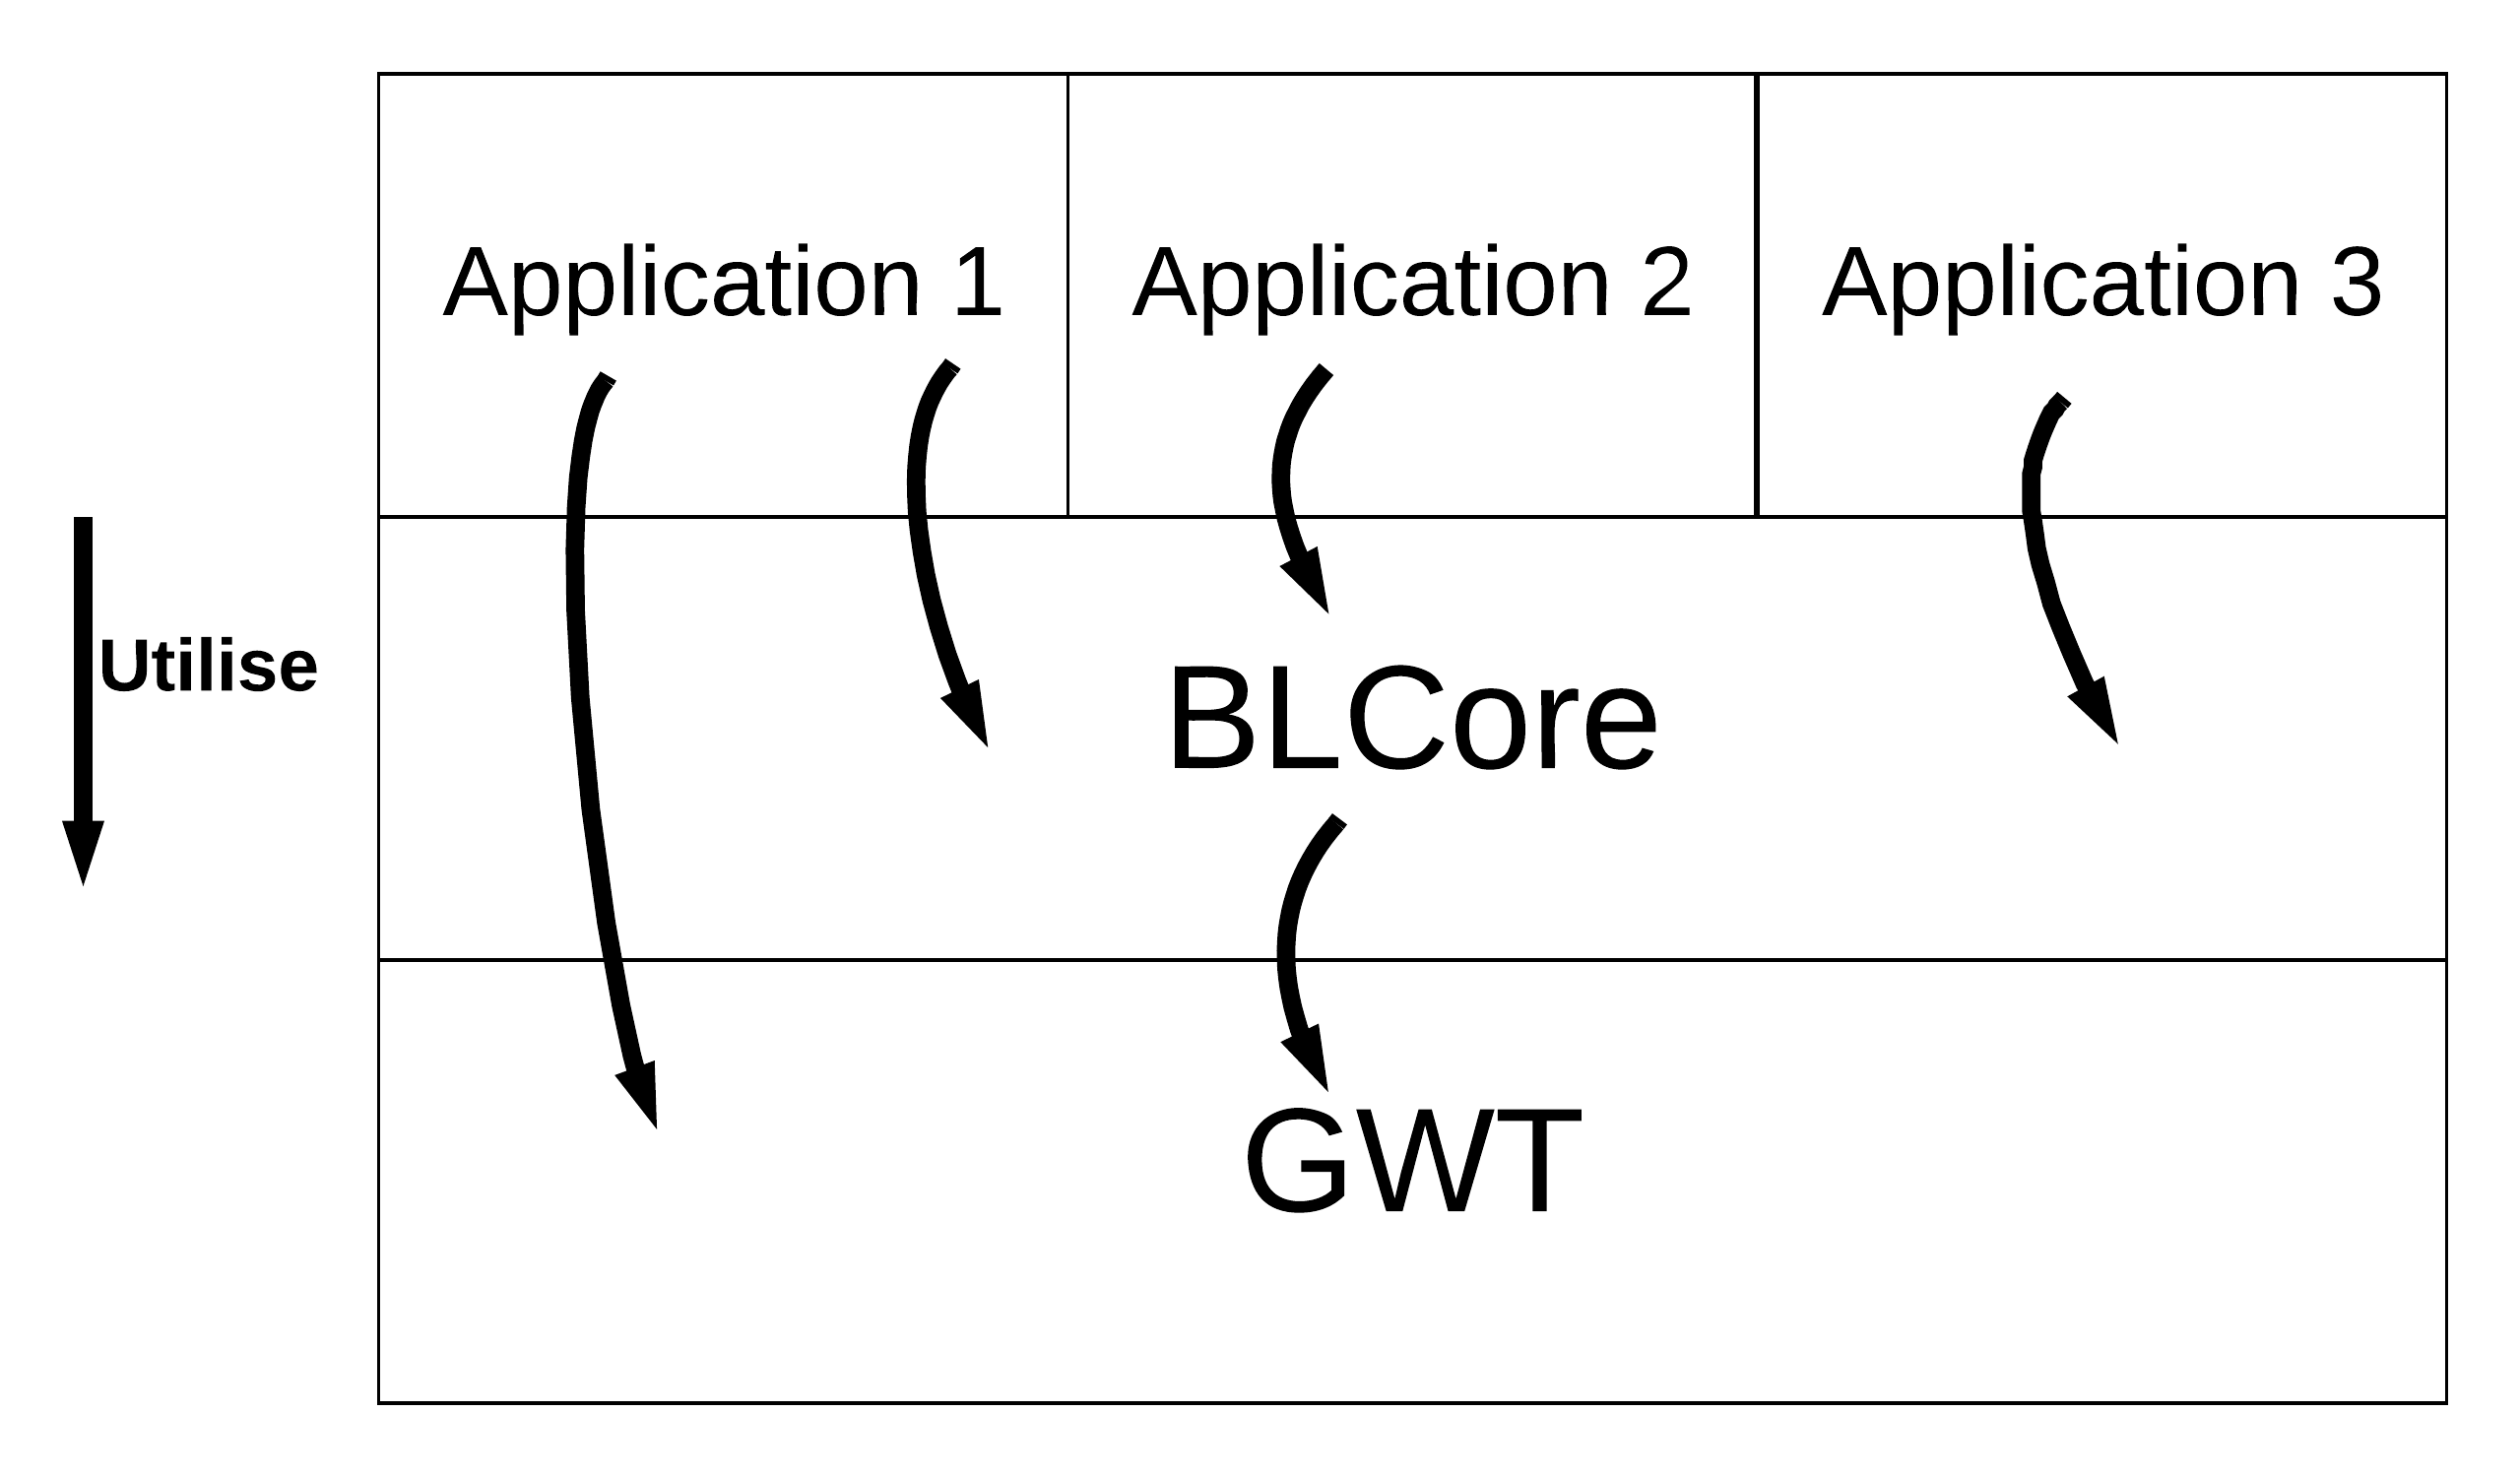
\includegraphics[width=2.60417in,height=2.60417in]{figures/structure.png}
\caption{Structure application}\label{architectureBL}
\end{figure}
}

Les applications de Berger-Levrault sont complexes. Ce sont les plus
importantes applications GWT en terme de ligne de code et de classes
dans le monde. Elles définissent plusieurs centaines de pages web. Bien
qu'une migration complète de l'application en réécrivant l'ensemble du
code est possible, c'est une tâche coûteuse et sujette à erreurs.
Automatiser toute la migration semble donc être la bonne solution,
cependant les développeurs ne seront pas formés sur la nouvelle
technologie et sur son utilisation dans les nouvelles applications. Le
manque de connaissance du langage cible va ralentir les développements
et peut faire \emph{peur} aux développeurs qui pourrait refuser une
telle solution. Une alternative pour contourner ce problème serait de
créer des outils facilitant la migration et en migrer une partie de
l'application. Les développeurs pourront alors effectuer la fin de la
migration rapidement et seront formés sur le nouveau langage et sur
l'application en le pratiquant assisté de nos outils.

La complexité de la migration des applications de Berger-Levrault réside
dans leurs tailles mais aussi et surtout dans le changement de langage.
En effet, les applications sont développées intégralement en Java tout
comme le framework GWT. Or, pour utiliser Angular 6, le programme doit
être écrit en TypeScript. La question qui se pose est de savoir quelle
couche de la Figure \ref{architectureBL} nous devons migrer et comment ?

En plus des difficultés techniques inherentes à un tel projet, une
entreprise comme Berger-Levrault a aussi des contraintes provenant de
leurs développeurs et de leurs clients. Parmi ces contraintes, la
migration devra, entre autre, conserver l'architecture sur laquelle se
base les applications de Berger-Levrault et ne pas perturber les clients
de Berger-Levrault du point de vue visuel des applications et
comportemental.

Mon objectif est donc de trouver des solutions pour aider à la migration
des applications de Berger-Levrault, de les évaluer et d'implémenter la
meilleure solution respectant les contraintes de l'entreprise. Pour
cela, j'ai dans un premier temps étudié la structure d'une application
de Berger-Levrault. Puis, j'ai défini avec un expert Angular
l'architecture attendu pour les applications post-migration. Ensuite,
j'ai définie une stratégie pour faire la migration en m'inspirant d'une
étude de l'état de l'art que j'ai menée. Enfin, j'ai commencé le
développement d'une suite d'outil permettant de mettre en application la
stratégie définie et l'évaluer.

J'ai effectué cette étude sur l'application \emph{bac-à-sable} de
Berger-Levrault. Cette dernière permet aux employés de Berger-Levrault
de consulter les éléments disponibles depuis BLCore. Bien que plus
petite que les applications en production, elle contient tout de même
plusieurs centaines de classes. Cependant, j'ai régulièrement vérifier
que mon travail pouvait s'appliquer sur les projets plus important de
Berger-Levrault.

\newpage

\hypertarget{etat-de-lart}{%
\section{Etat de l'art}\label{etat-de-lart}}

La première étape de mon travail a été de le positionner par rapport à
la littérature existante.

\hypertarget{migration-de-plateforme}{%
\subsection{Migration de plateforme}\label{migration-de-plateforme}}

La \emph{migration de plateforme} traite de comment migrer une interface
graphique.

En particulier, l'article de Samir \emph{et al.} {[}1{]} dans lequel il
est question de la migration de Swing vers Ajax. Les auteurs ont
développé un outil appelé Swing2Script qui permet d'automatiser la
migration d'application Java-Swing en une application web Ajax. Cet
outil permet d'extraire depuis une application Java les différentes
fenêtres et de les transcrire au format XUL\footnote{XUL: XML-based User
  interface Language est un langage de description d'interfaces
  graphiques fondé sur XML créé dans le cadre du projet Mozilla}.
Ensuite, l'outil ajoute à chacun des fichiers un fichier JavaScript
contenant l'ensemble des fonctions pouvant être appelées. Cependant,
l'outil utilise une analyse dynamique de l'application pour détecter son
fonctionnement. Au vu de la taille des applications de Berger-Levrault
ainsi que de l'impact de l'utilisation d'une telle stratégie sur les
utilisateurs, je ne pourrai pas utiliser la même stratégie.

L'article de Staiger {[}2{]} présente un outil d'analyse statique de
code source en C qui permet d'extraire l'interface graphique générée par
le programme. Pour cela, l'outil va rechercher les constructeurs de
composant graphique dans le code et leurs appellent. Il va ensuite
``suivre'' les pointeurs (C) pour detecter les ajouts de composants dans
d'autres composants. Ainsi, il arrive à créer un modèle de l'interface
graphique avec l'ensemble des widgets. L'outil permet aussi de récupérer
les événements liés aux composants détectés. Dans la cas d'utilisation
d'un modèle pour la migration des applications de Berger-Levrault, ce
travail peut nous permettre d'extraire le modèle contenant les
informations vis-à-vis de la représentation graphique de l'application.

Morgado \emph{et al.} {[}3{]} ont créé un outil permettant d'extraire
les différents composants d'une interface graphique ainsi que les
changements qui s'opèrent lorsque l'on effectue une action sur un
composant. Pour cela, les auteurs ont utilisé une stratégie de recherche
dynamique. Une fois lancée sur une interface en cours d'exécution, le
logiciel va détecter tous les composants graphiques. Puis, il va
exécuter des cliques sur les composants de l'interface et détecter les
modifications apportées à cette dernière. Comme Berger-Levrault souhaite
conserver la même interface graphique, je vais aussi avoir besoin
d'extraire la structure de l'interface actuelle. L'outil développait par
les auteurs peut peut-être s'appliquer à notre problématique ou nous
guider pour la création d'une solution.

L'article de Shah \emph{et al.} {[}4{]} présente un logiciel capable
d'extraire l'interface graphique d'une application java pendant
l'execution. Le logiciel récupère dans la mémoire de l'ordinateur
l'architecture de l'interface graphique avec la composition des widgets.
De cette manière, les auteurs arrivent à concevoir, pour chaque
``écran'' de l'application, un modèle contenant les informations sur
l'interface graphique. C'est-à-dire, les différents widgets, leurs
propriétés, la composition d'un widget avec un autre (ex: un panel qui
contient du text, un autre panel et un bouton). Comme les auteurs, la
migration des applications de Berger-Levrault peut nécessiter que l'on
extrait les interfaces graphiques des logiciels. La stratégie
d'extraction présentée dans l'article peut guider notre travail.

Sánchez Ramón \emph{et al.} {[}5{]} ont développé une solution
permettant d'extraire depuis un ancien logiciel son interface graphique.
Les auteurs importent cette interface dans un modèle qu'ils ont créé.
Leur solution permet ensuite d'extraire des informations de leur modèle.
Pour cela, l'outil va délimiter pour chaque widget la taille de sa
représentation visuelle. Il connaît donc, la position, la largeur et la
hauteur de chaque widget. Les widgets sont alors contenus ou non dans un
autre en fonction de leurs positions les uns avec les autres. Exemple :
un widget qui est à l'intérieur d'un autre visuellement est un contenu
par cet autre. Ce travail se rapproche de celui que nous devons
effectuer pour la migration des applications de Berger-Levrault.
Extraire l'interface graphique pour ensuite la migrer fait aussi partie
des tâches essentielles de notre migration. Le modèle représentant
l'interface graphique utilisé par les auteurs peut être un point de
départ à notre travail d'extraction.

Silvia \emph{et al.} {[}6{]} ont créé un logiciel nommé ``GUISurfer''.
Ce logiciel permet d'extraire une interface graphique d'un code source
et de le convertir en un modèle. Le code source peut être du java avec
le framework Swing. GUISurfer parcourt l'AST{[}\^{}ast{]} de
l'application source pour détecter les composants qu'on lui a donnés en
paramètre. On peut donc avoir en sortie un modèle complet de l'interface
graphique ou ne contenant que les actions (entrée, clique, etc.).
L'article précise qu'un travail sur l'extraction d'interface GWT est en
cours. Pour la migration des applications de Berger-Levrault, je vais
devoir extraire l'interface graphique des applications écrites avec GWT.
Le logiciel ``GUISurfer'' peut peut-être me permettre d'extraire un
modèle de l'interface, dans un premier temps sans les spécificités de
Berger-Levrault.

L'article de Gotti \emph{et al.} {[}7{]} présente une méthodologie pour
extraire les composants d'une interface graphique et leurs relations.
Pour cela, les auteurs construisent plusieurs modèles. Le passage entre
les modèles se fait grâce à des transformations QVT\footnote{QVT est un
  langage permettant de définir des transformation de modèle.}. Les
auteurs ont appliqué leur projet sur des programmes java utilisant le
framework graphique Swing. Dans le cadre de la migration des
applications de Berger-Levrault, l'extraction des composants graphiques
et de leurs relations peut être nécessaire. En modifiant le travail des
auteurs, je pourrai le réutiliser dans le cas de l'extraction de
composant GWT.

Memon \emph{et al.} {[}8{]} ont développé un logiciel nommé ``GUI
Ripper''. Cet outil permet d'extraire d'un logiciel java ou MS Windows
les différents composants visuels. L'outil fait une recherche dynamique
des composants instanciés durant l'exécution du programme. Les auteurs
obtiennent un modèle de l'application qu'ils vont ensuite pouvoir
utiliser pour générer des tests. L'extraction de composants visuels est
aussi une tâche importante pour mon projet avec Berger-Levrault.
Cependant, la recherche dynamique proposée par les auteurs ne semblent
pas applicable en l'état dans notre cas puisque nous n'avons pas
d'exécution de l'interface, mais sa compilation par GWT. Cependant, on
peut imaginer implémenter l'algorithme de GUI Ripper en JavaScript pour
extraire les widgets pendant l'exécution du script dans le navigateur
web.

L'article de Lelli \emph{et al.} {[}9{]} propose un outil permettant de
détecter les composants graphiques pouvant faire plus de deux actions.
L'outil, qui est une extension d'eclipse, va tout d'abord faire une
analyse statique du code source. Cela lui permet de repérer les
différents widgets. Puis il va détecter les widgets qui ont plus de deux
ajout de Listener. Puisque le plugin est capable de détecter les ajout
de listener, il doit être capable de détecter les ajouts d'autres
widgets. Nous pourrions donc modifier le plugin pour qu'il détecte en
plus les compositions de widgets afin d'extraire un modèle contenant
l'aspect graphique des applications de Berger-Levrault. Cette dernière
étape nous sera utile pour migrer correctement les applications.

Cloutier \emph{et al.} {[}10{]} ont conçu un outil nommé ``Wavi'' qui
permet d'extraire d'une page web les différents composants. Pour cela,
l'outil se base sur les fichier html, css et JavaScript. L'outil va dans
un premier temps construire l'arbre syntaxique du code source du site
web. Puis il extrait les éléments importants du fichier html
(\emph{i.e.} les hyperliens, formulaires, appel JavaScript, etc. ).
Enfin il va relier les éléments de l'étape une et deux. Les applications
web de Berger-Levrault sont développées en java avec GWT, mais une fois
compilées sont des fichiers html, css et JavaScript. Toutes les
conditions semblent donc remplit pour pouvoir utilise le travail des
auteurs dans notre cas et ainsi extraire l'architecture des applications
de Berger-Levrault. Ce travail est nécessaire si l'on souhaite conserver
la même structure visuelle pendant la migration.

Aho \emph{et al.} {[}11{]} ont développé un logiciel appelé ``Murphy''.
Murphy permet d'extraire dynamiquement les widgets d'une application.
Murphy est compatible avec de nombreux langages de programmation car il
utilise des ``drivers'' qui lui permettent d'interagir avec
l'application en cours de fonctionnement grâce à une interface abstraite
du langage de programmation de l'application. Le projet des auteurs se
rapprochent du nôtre puisqu'ils souhaitent extraire l'interface
graphique ce qui est une de nos tâches pour la migration des
applications de Berger-Levrault. Il nous faudrait cependant trouver
comment créer un ``driver'' qui permettrait à Murphy d'interagir avec
une application web.

\hypertarget{migration-de-librairie}{%
\subsection{Migration de librairie}\label{migration-de-librairie}}

La \emph{migration de librairie} présente des solutions sur comment
changer de framework.

Teyton \emph{et al.} {[}12{]} ont proposé un outil permettant d'extraire
depuis des migrations déjà effectuées les correspondances entre les
appels d'un framework avec ceux d'un autre. Pour cela, ils se basent sur
les différences textuelles entre plusieurs versions d'un même projet. À
cause du nombre de versions qu'un projet peut avoir, ils utilisent un
algorithme ``diviser pour régner'' afin d'accélérer le temps de calcul.
Ce travail peut nous servir une fois que BLCore aura migré, afin
d'automatiser ou créer des outils facilitant le travail des
développeurs. Cependant, ce travail ne parle que de la migration au sein
d'un même langage de programmation. Il ne peut donc être utilisé tel
quel pour faire migrer BLCore de GWT vers Angular 4.

L'article de Hora \emph{et al.} {[}13{]} explique une démarche pour
extraire automatiquement des modifications faites dans un code afin d'en
déduire des pattern. Son objectif est de détecter les conventions de
développement qui évoluent. Son travail de recherche de correspondance
entre certains morceaux de code et des nouveaux peut m'être utile pour
la migration. En effet, je vais aussi devoir trouver les correspondances
entre du code Java et du code Angular.

Zhong \emph{et al.} {[}14{]} ont voulu créer une approche visant à faire
correspondre l'API\footnote{API: Interface de programmation} d'un
framework avec celui d'un autre, tous deux étant écrits dans des
langages différents. Pour cela, ils ont développé une stratégie appelée
MAM (Mining API Mapping) qui prendra en paramètres deux projets dans
deux versions différentes. Ensuite, l'algorithme essaie de regrouper par
minage les éléments identiques des deux projets (\emph{i.e.} les
classes, les méthodes). Puis il construit un arbre d'exécution pour les
méthodes et cherche les correspondances entre les méthodes qui sont
appelées. Cette approche ne peut pas m'aider à migrer BLCore, mais, si
je migre quelques applications de Berger-Levrault, je pourrai réutiliser
les stratégies employées par Zhong pour faciliter la migration d'autres
applications.

Nguyen \emph{et al.} {[}15{]} ont travaillé sur un outil, nommé
StaMiner, permettant de mettre en correspondance des API de framework
écrit en Java, avec des API écrite en C\#. L'apprentissage des
correspondances utilisent des morceaux de code source et cible ayant le
même comportement. Il se fait en trois étapes.

\begin{enumerate}
\def\labelenumi{\arabic{enumi}.}
\tightlist
\item
  Le Groum, qui consiste à représenter le code source sous la forme d'un
  graphe. On y retrouve les appels à des fonctions, des alternatives,
  des boucles, etc.
\item
  L'extraction des séquences d'utilisation des différents éléments.
\item
  L'alignement des séquences entre le résultat pour le code source et le
  code cible.
\end{enumerate}

Pour effectuer l'alignement, les auteurs ont utilisé des outils
probabilistes sur les symboles et sur les séquences. Ce travail peut
être utilisé pour la migration des applications de Berger-Levrault. En
utilisant cet outil sur une application source et un bout migration
\emph{fait à la main}, je pourrai apprendre des règles de transformation
à appliquer sur la migration.

L'article de Phan \emph{et al.} {[}16{]} décrit une manière de faire
correspondre des éléments de code du langage Java vers le langage C\#.
Plus précisément, ils ont développé un outil permettant de mettre en
correspondance du code d'un langage utilisant une ou plusieurs API vers
un autre langage utilisant une ou plusieurs autres API prédéfinies. Pour
cela, les auteurs utilisent un outil de recherche de correspondances
entre des API provenant de Java vers C\#. Puis, ils utilisent une
machine statistique de traduction automatique pour faire correspondre
les utilisations des API Java et C\#. Une fois le modèle entraîné, ils
arrivent à automatiser une partie de la migration. Ce travail peut nous
servir si l'on a migré BLCore et que l'on souhaite ensuite migrer les
applications. Comme lui, nous travaillons sur la migration de librairies
de langages différents.

Chen \emph{et al.} {[}17{]} ont développé un outil permettant de trouver
des librairies similaires à une autre. Pour cela, les auteurs ont miné
les tags des questions de Stack Overflow. Avec ces informations, ils ont
pu mettre en relation des langages et leurs libraries ainsi que des
équivalences entre librairies de langage différent. Pour la migration de
Java/GWT vers Angular, il est possible que nous ayons besoin de changer
de librairie (qui n'est pas BLCore). Plutôt que de récrire la librairie,
la recherche d'une autre librairie permettant de résoudre les même
problème peut être une solution. C'est dans ce contexte que le travail
des auteurs peut guider notre recherche de librairie en mettant faisant
correspondre les anciennes librairies utilisées par les applications de
Berger-Levrault avec d'autre compatible utilisable avec Angular.

\hypertarget{transformation-de-moduxe8le-vers-moduxe8le}{%
\subsection{Transformation de modèle vers
modèle}\label{transformation-de-moduxe8le-vers-moduxe8le}}

La \emph{transformation de modèle vers modèle} traite de la modification
d'un modèle source vers un modèle cible.

L'article de Baki \emph{et al.} {[}18{]} présente un processus de
migration d'un modèle UML vers un modèle SQL. Pour faire la migration,
les auteurs ont décidé d'utiliser des règles de transformation. Ces
règles prennent en entrée le modèle UML et donne en sortie le SQL
définit par les règles. Plutôt que d'écrire les règles de migration à la
main. Les auteurs ont décomposé ces règles en petites briques. Chaque
brique peut correspondre soit à une condition à respecter pour que la
règle soit validée, soit à un changement sur la sortie de la règle.
Ensuite, les auteurs ont développé un algorithme de programmation
génétique pouvant manipuler ces règles. L'algorithme va, à partir
d'exemples, apprendre les règles de transformation à appliquer afin
d'effectuer la transformation du modèle. Pour cela, il va modifier les
petites briques composants les règles et analyser si le modèle en sortie
ressemble à celui explicité pour tous les exemples. Puis, il sera
utilisé sur de vrais données. Ce travail peut être utilisé dans mon
projet. En effet, je peux aussi effectuer la migration en utilisant un
modèle de l'application source et un modèle de l'application cible.
Toutefois, la complexité d'un code source Java semble plus grande que
celle d'un modèle UML. Il est possible que l'algorithme de programmation
génétique ne soit pas assez performant pour régler mon problème de
manière satisfaisante.

Falleri \emph{et al.} {[}19{]} ont travaillé sur le passage d'un
méta-modèle à un autre. C'est ce que l'on appelle l'alignement des
méta-modèle. Pour cela, les auteurs ont utilisé l'algorithme de
\emph{Similarity Flooding}. Cet algorithme permet de trouver les
similarités entre les deux graphe orientés et étiquetés aux arcs en
entré du programme. Les auteurs ont proposé des solutions pour convertir
un méta-modèle en graphe orientés et étiquetés aux arcs. Comme les
auteurs, je peux décider d'effectuer la migration en passant par des
modèles et méta-modèles. Une fois les méta-modèle et modèles créés, je
pourrai utiliser l'algorithme \emph{Similarity Flooding} utilisée dans
l'article pour effectuer la migration.

Wang \emph{et al.} {[}20{]} ont créé une méthodologie et un outil
permettant d'automatiquement faire la transformation d'un modèle vers un
autre modèle. Leur outil se distingue en effectuant une migration qui se
base sur une analyse syntaxique et sémantique. L'objectif de la
méthodologie est d'effectuer la transformation d'un modèle vers un autre
de manière itérative en modifiant le méta-modèle. Une condition
d'utilisation contraignante décrite par les auteurs est la nécessité
d'avoir une méta-méta-modèle pour tous les méta-modèle intermédiaire.
Les auteurs ont implémenté un méta-méta-modèle dans leur outil. Dans mon
travail, une solution pour effectuer la migration serait d'utiliser des
méta-modèle. Le premier modèle proviendrait de l'application source, le
second modèle respecterait le méta-modèle de destination. J'ai donc la
même problématique que les auteurs de passage d'un modèle à un autre. En
définissant un méta-méta-modèle que respecterai le méta-modèle de départ
de l'application source et un méta-modèle de destination, la
méthodologie proposée par les auteurs devrait pouvoir résoudre,
totalement ou partiellement, mon problème de migration.

Fleurey \emph{et al.} {[}21{]} ont travaillé sur la modernisation et la
migration de logiciel au sein d'une entreprise d'informatique. Ils ont
développé un logiciel permettant de semi-automatiser la migration des
applications de l'entreprise. Pour cela, ils ont utilisé la
transformation de modèle sur trois modèles. La migration se passe en
quatre étapes.

\begin{enumerate}
\def\labelenumi{\arabic{enumi}.}
\tightlist
\item
  Ils génèrent un modèle de l'application à migrer.
\item
  Ils transforment ce modèle en un ``modèle pivot''. Ce dernier contient
  la structure des données, les actions et algorithmes, l'interface
  graphique et la navigation dans l'application.
\item
  Ils transforment le modèle pivot en un modèle respectant le
  méta-modèle du langage cible.
\item
  Ils génèrent le code source final de l'application.
\end{enumerate}

Comme les auteurs, je vais devoir faire la migration d'une application
et je vais devoir conserver structure de données, actions, interface
graphique et navigation dans l'application. Mon travail peut donc
s'inspirer de celui proposé par les auteurs si nous souhaitons utiliser
les modèles pour effectuer la migration.

L'article de Garcés \emph{et al.} {[}22{]} décrit les trois étapes que
les auteurs ont suivies pour effectuer une migration d'anciens codes.

\begin{enumerate}
\def\labelenumi{\arabic{enumi}.}
\tightlist
\item
  L'analyse de l'ancien code source pour créer un modèle de
  l'application suivant un méta-modèle. Ce premier modèle est proche de
  la technologie de départ.
\item
  La transformation de ce modèle vers un nouveau modèle plus abstrait.
\item
  La génération du nouveau code source depuis le dernier modèle.
\end{enumerate}

Comme pour l'article, le travail de migration de Berger-Levrault peut se
faire en utilisant des modèles et méta-modèles. De plus, les auteurs ont
travaillé sur une migration d'interface graphique ce qui est aussi notre
besoin. Nous pourrions donc réutiliser des outils ou résultats de ce
travail dans notre cas.

\hypertarget{transformation-de-moduxe8le-vers-texte}{%
\subsection{Transformation de modèle vers
texte}\label{transformation-de-moduxe8le-vers-texte}}

La \emph{transformation de modèle vers texte} traite du passage d'un
modèle source vers du texte. Le texte peut être du code source
compilable ou non.

L'article de Mukherjee \emph{et al.} {[}23{]} présente un outil
permettant de prendre en entrée les spécifications d'un programme et
donne en sortie un programme utilisable. L'entrée est un fichier en XML
et la sortie est un programme écrit en C ou en Java (en fonction du
choix de l'utilisateur). Pour effectuer les transformations, les auteurs
ont utilisé un système de règles de transformation. Je pourrai
réutiliser ce travail si je passe par un modèle pour la migration. En
effet, le fichier XML pris en entrée de l'outil des développeurs peut
être assimilé à un modèle suivant un méta-modèle (définit dans
l'article). Dans le cas où nous utilisons un modèle dans le cadre de la
migration des applications de Berger-Levrault. Nous pourrions aussi être
amené à utiliser un système de règle pour faire la migration du modèle
au code source.

\hypertarget{migration-de-langage}{%
\subsection{Migration de langage}\label{migration-de-langage}}

La \emph{migration de langage} traite de la transformation du code
source directement (\emph{i.e.} sans passer par un modèle). Pour cela,
les auteurs créent des ``règles'' permettant de modifier le code source.

Brant \emph{et al.} {[}24{]} ont écrit un compilateur utilisant un outil
nommé SmaCC. SmaCC est un générateur d'analyseur pour Smalltalk. Ils ont
aussi utilisé le SmaCC Transformation Toolkit qui permet de définir des
règles de transformations qui seront utilisées par SmaCC. Ainsi, les
auteurs sont parvenues à migrer une application Delphi de 1,5 million de
lignes de code en C\#. Comme les auteurs, je veux effectuer la migration
du code source d'une application. Mon cas se différencie par les
langages source et cible. Ce travail peut me servir si nous souhaitons
effectuer la migration sans passer par un modèle intermédiaire.

Un des problèmes de la migration du code source est la définition des
règles. Newman \emph{et al.} {[}25{]} ont proposé un outil facilitant la
création de règle de transformation. Pour cela, l'outil va
``normaliser'' le code source en entré et essayer de le simplifier.
Ainsi, les auteurs arrivent à réduire le nombre de règles de
transformations à écrire et leurs complexités. Dans le cas de migration
de Berger-Levrault. J'aurai à gérer les multiples manières dont les
fonctionnalités seront écrites. La normalisation du code source pourra
simplifier l'écriture des règles de transformation ou les règles
permettant de créer un modèle.

Rolim \emph{et al.} {[}26{]} ont créé un outil qui apprend des règles de
transformation de programme à partir d'exemple. Pour cela, les auteurs
ont défini un DSL\footnote{DSL: Domain Specific Language est un langage
  de programmation destiné à générer des programme dans un domaine
  spécifique.} permettant d'exprimer les modification faîte sur
l'AST{[}\^{}ast{]} d'un programme. Ensuite, à partir d'une base
d'exemple de transformation, l'outil recherche les règles de
transformation entre les fichiers d'entrés des exemples et ceux de
sorties. Une fois les règles trouvées et écrites dans le DSL prédéfini,
l'outil prend en entré un bout de code et donne en sortie le résultat
des transformation. Ce travail peut nous servir pour la migration des
applications de Berger-Levrault. En effet, nous pouvons imaginer faire
la migration de tout ou partie des applications en utilisant un tel
outil. De plus, on peut imaginer un outil qui apprendrai au fur et à
mesure des développement des développeur et qui les conseillerez dans un
second temps sur d'autre développement avec les même problématiques déjà
résolu. Ou encore, l'outil pourrait servir de ``guide'' pour les
nouveaux développeurs participants à la migration ou au développement
courant des applications.

Aucun des papiers trouvés et cités ne peut nous aider réellement à
migrer le framework BLCore ou les applications si on décide que dans le
futur, on supprime BLCore, puisqu'Angular, contrairement à GWT n'est pas
du Java. En revanche, si Berger-Levrault souhaite garder l'équivalent de
BLCore dans le futur, alors ces travaux pourraient nous aider à migrer
dans un deuxième temps les applications.

\newpage

\hypertarget{gui-duxe9composition}{%
\section{GUI Décomposition}\label{gui-duxe9composition}}

Les applications que nous devons migrer ont des interfaces graphiques.
Avant de créer l'outil de migration, il faut comprendre ce qu'est une
telle interface et comment nous pouvons la diviser. Diviser un problème
en petits sous-problèmes est une méthode efficace pour résoudre des
problèmes complexes. Nous avons identifié trois parties dans une
interface graphique :

\begin{itemize}
\tightlist
\item
  L'interface utilisateur
\item
  Le code de l'entreprise
\item
  Le code comportemental
\end{itemize}

\hypertarget{interface-utilisateur}{%
\subsection{Interface utilisateur}\label{interface-utilisateur}}

L'interface utilisateur est la partie visible. Cet élément représente
l'interface de l'application. Elle comprend les composants de
l'interface. L'interface utilisateur ne contient pas la visualisation
exacte d'un composant, mais elle peut préciser certaines
caractéristiques inhérentes au composant, comme la possibilité d'être
cliqué, ~~~~ou certaines propriétés du composant, comme sa couleur ou sa
taille. Plus que les composants, elle décrit également la disposition
~~~~de ces composants par rapport aux autres. Dans le cas où une
application est composée de plusieurs fenêtres (ou de pages web pour une
application web), ~~~~l'interface utilisateur contient toutes les
fenêtres.

\hypertarget{code-comportemental}{%
\subsection{Code comportemental}\label{code-comportemental}}

Le code comportemental est la partie \emph{executable} de l'application.
Cela correspond à la logique de l'application. Il peut avoir deux
manifestations du code comportemental. Il peut être exécuté soit par une
action de l'utilisateur sur un composant d'interface (comme un clic) ou
par le système lui-même. Comme un langage de programmation
\emph{``classique''}, le code métier contient des structures de contrôle
(\emph{i.e.} boucle et alternative). Lié à l'interface utilisateur, le
code comportemental définit la logique de l'interface utilisateur.
Cependant, le code comportemental n'exprime pas la logique de
l'application. Cette partie est dédiée au code comportemental.

\hypertarget{code-muxe9tier}{%
\subsection{Code métier}\label{code-muxe9tier}}

Le code métier définit les informations spécifiques d'une application.
Il est composé par les règles générales de l'application (comment
calculer les taxes ?), le lien services distants (quel serveur mon code
métier doit demander), les données de l'application (quelle base de
données ? quel type de \emph{object}). Le code métier n'est donc pas
directement lié à l'interface utilisateur.

\newpage

\hypertarget{description-du-probluxe8me-1}{%
\section{Description du problème}\label{description-du-probluxe8me-1}}

Dans le contexte de l'évolution des applications de Berger-Levrault,
l'entreprise a estimé la transformation du code à X jours de
développement. Ceci s'explique majoritairement par les 1,67
MLOC\footnote{MLOC : Million lines of code} utilisés pour les logiciels.
Un de mes objectifs à Berger-Levrault est de définir une stratégie de
migration qui réduit le temps nécessaire pour la transformation des
programmes.

\hypertarget{contraintes}{%
\subsection{Contraintes}\label{contraintes}}

Berger-Levrault étant une importante entreprise dans le domaine de
l'édition de logiciel, elle a des contraintes spécifiques vis-à-vis d'un
outil de migration. En effet, la solution logicielle que j'ai produite
doit respecter les contraintes suivantes :

\begin{itemize}
\tightlist
\item
  \emph{Depuis GWT (BLCore)}. La solution doit au moins fonctionner dans
  le cas de Berger-Levrault. Elle peut être plus général mais ne doit
  pas faire de concession sur le résultat final.
\item
  \emph{Vers Angular}. Dans le cas d'une automatisation ou
  semi-automatisation du processus de migration, celle-ci doit s'achever
  par la génération de code Angular. La solution peut contenir des
  structures facilitant son utilisation pour d'autre langages cible mais
  pas au détriment du projet fixé avec Berger-Levrault.
\item
  \emph{Approche modulaire}. La migration doit être divisée en petites
  étapes. Cela permet de facilement remplacer une étape ou de l'étendre
  sans introduire d'instabilité. Cette contrainte est essentielle pour
  les entreprises qui désirent avoir un contrôle fin du processus de
  migration. L'approche modulaire permet entre autres aux entreprises de
  modifier l'implémentation de la stratégie pour respecter leurs
  contraintes spécifiques.
\item
  \emph{Préservation de l'architecture}. Après la migration, nous devons
  retrouver la même architecture entre les différents composants de
  l'interface graphique (\emph{c.-à-d.} un bouton qui appartenait à un
  panel dans l'application source appartiendra au même panel dans
  l'application cible). Cette contrainte permet de faciliter le travail
  de compréhension de l'application cible par les développeurs. En
  effet, ils vont retrouver la même architecture qu'ils avaient dans
  l'application source.
\item
  \emph{Préservation du visuel}. Il ne doit pas y avoir de différence
  visuelle entre l'application source et l'application cible. Cette
  contrainte est particulièrement importante pour les logiciels
  commerciaux. En effet, les utilisateurs de l'application ne doivent
  pas être perturbés par la migration.
\item
  \emph{Automatique}. La solution apportée doit être automatique. Les
  utilisateurs de l'outil ne devrait pas intervenir pendant le processus
  de migration ou très peu. Ainsi, l'outil peut être utilisé avec un
  minimum de connaissance préalable.
\item
  \emph{Amélioration de la qualité}. La migration doit permettre de
  traiter les possibles déviances du programme source. Par exemple, dans
  le cas de Berger-Levrault, l'outil de migration doit être capable de
  gérer les éléments utilisés par l'application à migrer et provenant du
  framework GWT. Cette exemple d'utilisation du framework GWT par
  l'Application 1 est représenté Figure \ref{architectureBL}.
\end{itemize}

Une dernière contrainte inhérent aux entreprises est la possibilité pour
les équipes de développement de continuer la maintenance des
applications pendant le développement de la stratégie de migration et la
migration elle-même.

\hypertarget{comparaison-de-gwt-et-angular}{%
\subsection{Comparaison de GWT et
Angular}\label{comparaison-de-gwt-et-angular}}

\begin{table}[hbtp]
    \caption{Comparaison des architectures de GWT et Angular}
    \label{comparaison}
    \begin {center}
    \resizebox{\columnwidth}{!}{%
    \begin{tabular}{|l|l|l|}
        \hline
         & GWT & Angular \\
        \hline
        Page web    & Une classe Java & Un fichier TypeScript et un fichier HTML \\
        \hline
        Style pour une page web & Inclus dans le fichier Java & Un fichier CSS optionnel \\
        \hline
        Nombre de fichiers de configuration & Un fichier de configuration & Quatre fichiers plus deux par sous-projets \\
        \hline
    \end{tabular} %
    }
    \end{center}
\end{table}

Dans le cas de ce projet, le langage de programmation source et cible
ont deux architectures différentes. Les différences sont syntaxicales,
semanticales et architecturales. Pour la migration d'application GWT
vers Angular, les fichier \emph{.java} sont séparés en plusieurs
fichiers Angular.

Le Tableau \ref{comparaison} synthétise les différences entre
l'architecture d'une application en java et celle en Angular. Les
différences se font pour trois notions, les pages web, leurs styles et
les fichiers de configuration.

Avec le Framework GWT, un seul fichier est nécessaire pour représenter
une page web. L'ensemble de la page web peut donc être contenu dans ce
fichier, il reste toutefois possible de créer d'autres fichiers pour
séparer les différents éléments de la page web. Les fichiers java
contiennent les différents widgets de la page web, leurs positions les
uns par rapport aux autres et leurs organisations hiérarchiques. Dans le
cas d'un widget sur lequel une action peut être exécutée (comme un
bouton), c'est dans ce même fichier qu'est contenu le code à executer
lorsque l'action est réalisée. En Angular, on crée une hiérarchie de
fichier correspondant à un \emph{sous-projet} pour chaque page web. Ce
sous-projet contient plusieurs fichiers dont un fichier HTML qui
contient les widgets de la page web et leurs organisations, et un
fichier TypeScript contenant le code à exécuter quand une action se
produit sur les widgets du fichier HTML. On a donc la séparation d-un
fichier java pour GWT vers deux fichiers HTML et TypeScript en Angular
pour représenter les widgets et le code qui leur sont associés.

Pour le style visuel d'une page web, dans le cas de GWT, il y a un
fichier CSS commun à toutes les pages web et des modifications qui sont
appliquées directement dans le fichier java de la page web. Ces
modifications peuvent porter sur la couleur ou les dimensions. En
Angular, on retrouve le même fichier CSS général pour tout le projet,
cependant, c'est un fichier CSS que l'on doit créer par sous-projet qui
va définir le visuel des éléments de la page web. Il y a donc création
d'un fichier supplémentaire en Angular par rapport à GWT.

Pour les fichiers de configurations, GWT n'a besoin que d'un fichier de
configuration qui définis les fichiers java correspondant à une page web
et les URL que l'on devra utiliser pour y accéder. En Angular, il y a
deux fichiers de configuration générale. Le premier, \emph{module},
explicite les différentes pages web accessible dans l'application ainsi
que les services distant et les composants graphiques (widgets)
utilisable dans l'application. Le second, de \emph{routing}, définit
pour les différentes pages web de l'application leurs chemins d'accès.

\hypertarget{sec:strategieMigration}{%
\subsection{Stratégies de migration}\label{sec:strategieMigration}}

Il existe plusieurs manières d'effectuer la migration d'une application.
Toutes les solutions doivent respecter les contraintes définies Section
\ref{contraintes}.

\hypertarget{exampleRuleEngine}{%
\begin{figure}
\centering
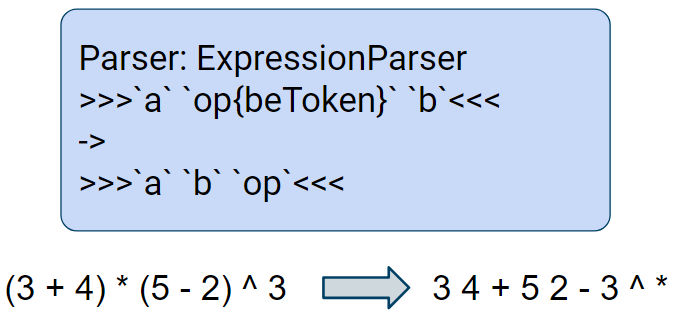
\includegraphics[width=3.64583in,height=2.60417in]{figures/exampleRuleEngine.png}
\caption{Exemple de règle de transformation}\label{exampleRuleEngine}
\end{figure}
}

\begin{itemize}
\tightlist
\item
  \emph{Migration manuelle}. Cette stratégie correspond au
  re-développement complet des applications sans l'utilisation d'outils
  aidant à la migration. La migration manuelle permet de facilement
  corriger les potentielles erreurs de l'application d'origine et de
  re-concevoir l'application cible en suivant les préceptes du langage
  cible.\\
\item
  \emph{Utilisation d'un moteur de règles}. L'utilisation d'un moteur de
  règles pour migrer partiellement ou en totalité une application a déjà
  été appliqué sur d'autres projets {[}24{]}, {[}27{]}, {[}28{]}. Pour
  utiliser cette stratégie, nous devons définir et créer des règles qui
  prennent en entrée le code source et qui produisent le code pour
  l'application migrée. La Figure \ref{exampleRuleEngine} montre un
  exemple de règle de transformation. Dans ce cas, elle permet de
  changer la position des opérateurs dans une expression mathématique
  source. L'opérateur est maintenant en suffixe de l'expression. Il est
  possible que la migration ne soit pas complète. Dans ce cas, les
  développeurs devront finir le processus de migration avec du travail
  manuel. L'utilisation d'un moteur de règles, bien qu'efficace,
  implique une solution qui n'est ni indépendante de la source, ni
  indépendante de la cible de la migration.
\item
  \emph{Migration dirigée par les modèles}. La migration dirigée par les
  modèles implique le développement de méta-modèles pour effectuer. La
  stratégie respecte l'ensemble des contraintes que nous avons défini.
  Une migration semi-automatique ou complètement automatique est
  envisageable avec cette stratégie de migration. Comme pour
  l'utilisation d'un moteur de règle, dans le cas d'une migration
  semi-automatique, il peut y avoir du travail manuel à effectuer pour
  compléter la migration.
\end{itemize}

\newpage

\hypertarget{mise-en-place-de-la-migration-par-via-les-moduxe8les}{%
\section{Mise en place de la migration par via les
modèles}\label{mise-en-place-de-la-migration-par-via-les-moduxe8les}}

Suite à l'étude des contraintes inhérentes aux problèmes de migration
dans le cadre d'une entreprise. Et après la recherche de l'état de
l'art. Nous avons travaillé sur la conception et l'implémentation d'une
stratégie de migration respectant les critères que nous avons fixés.

Comme vu Section \ref{sec:strategieMigration}, seule la migration en
utilisant les modèles nous permet de respecter toutes les contraintes.
Ce type de migration nous impose la conception de méta-modèles.

Nous allons présenter dans cette partie le processus de migration que
nous avons conçu, puis le méta-modèle d'interface utilisateur utilisé
dans le ce processus, et enfin expliquer l'implémentation de cette
stratégie.

\hypertarget{sec:processusMigration}{%
\subsection{Processus de migration}\label{sec:processusMigration}}

\hypertarget{fig:processusMigration}{%
\begin{figure}
\centering
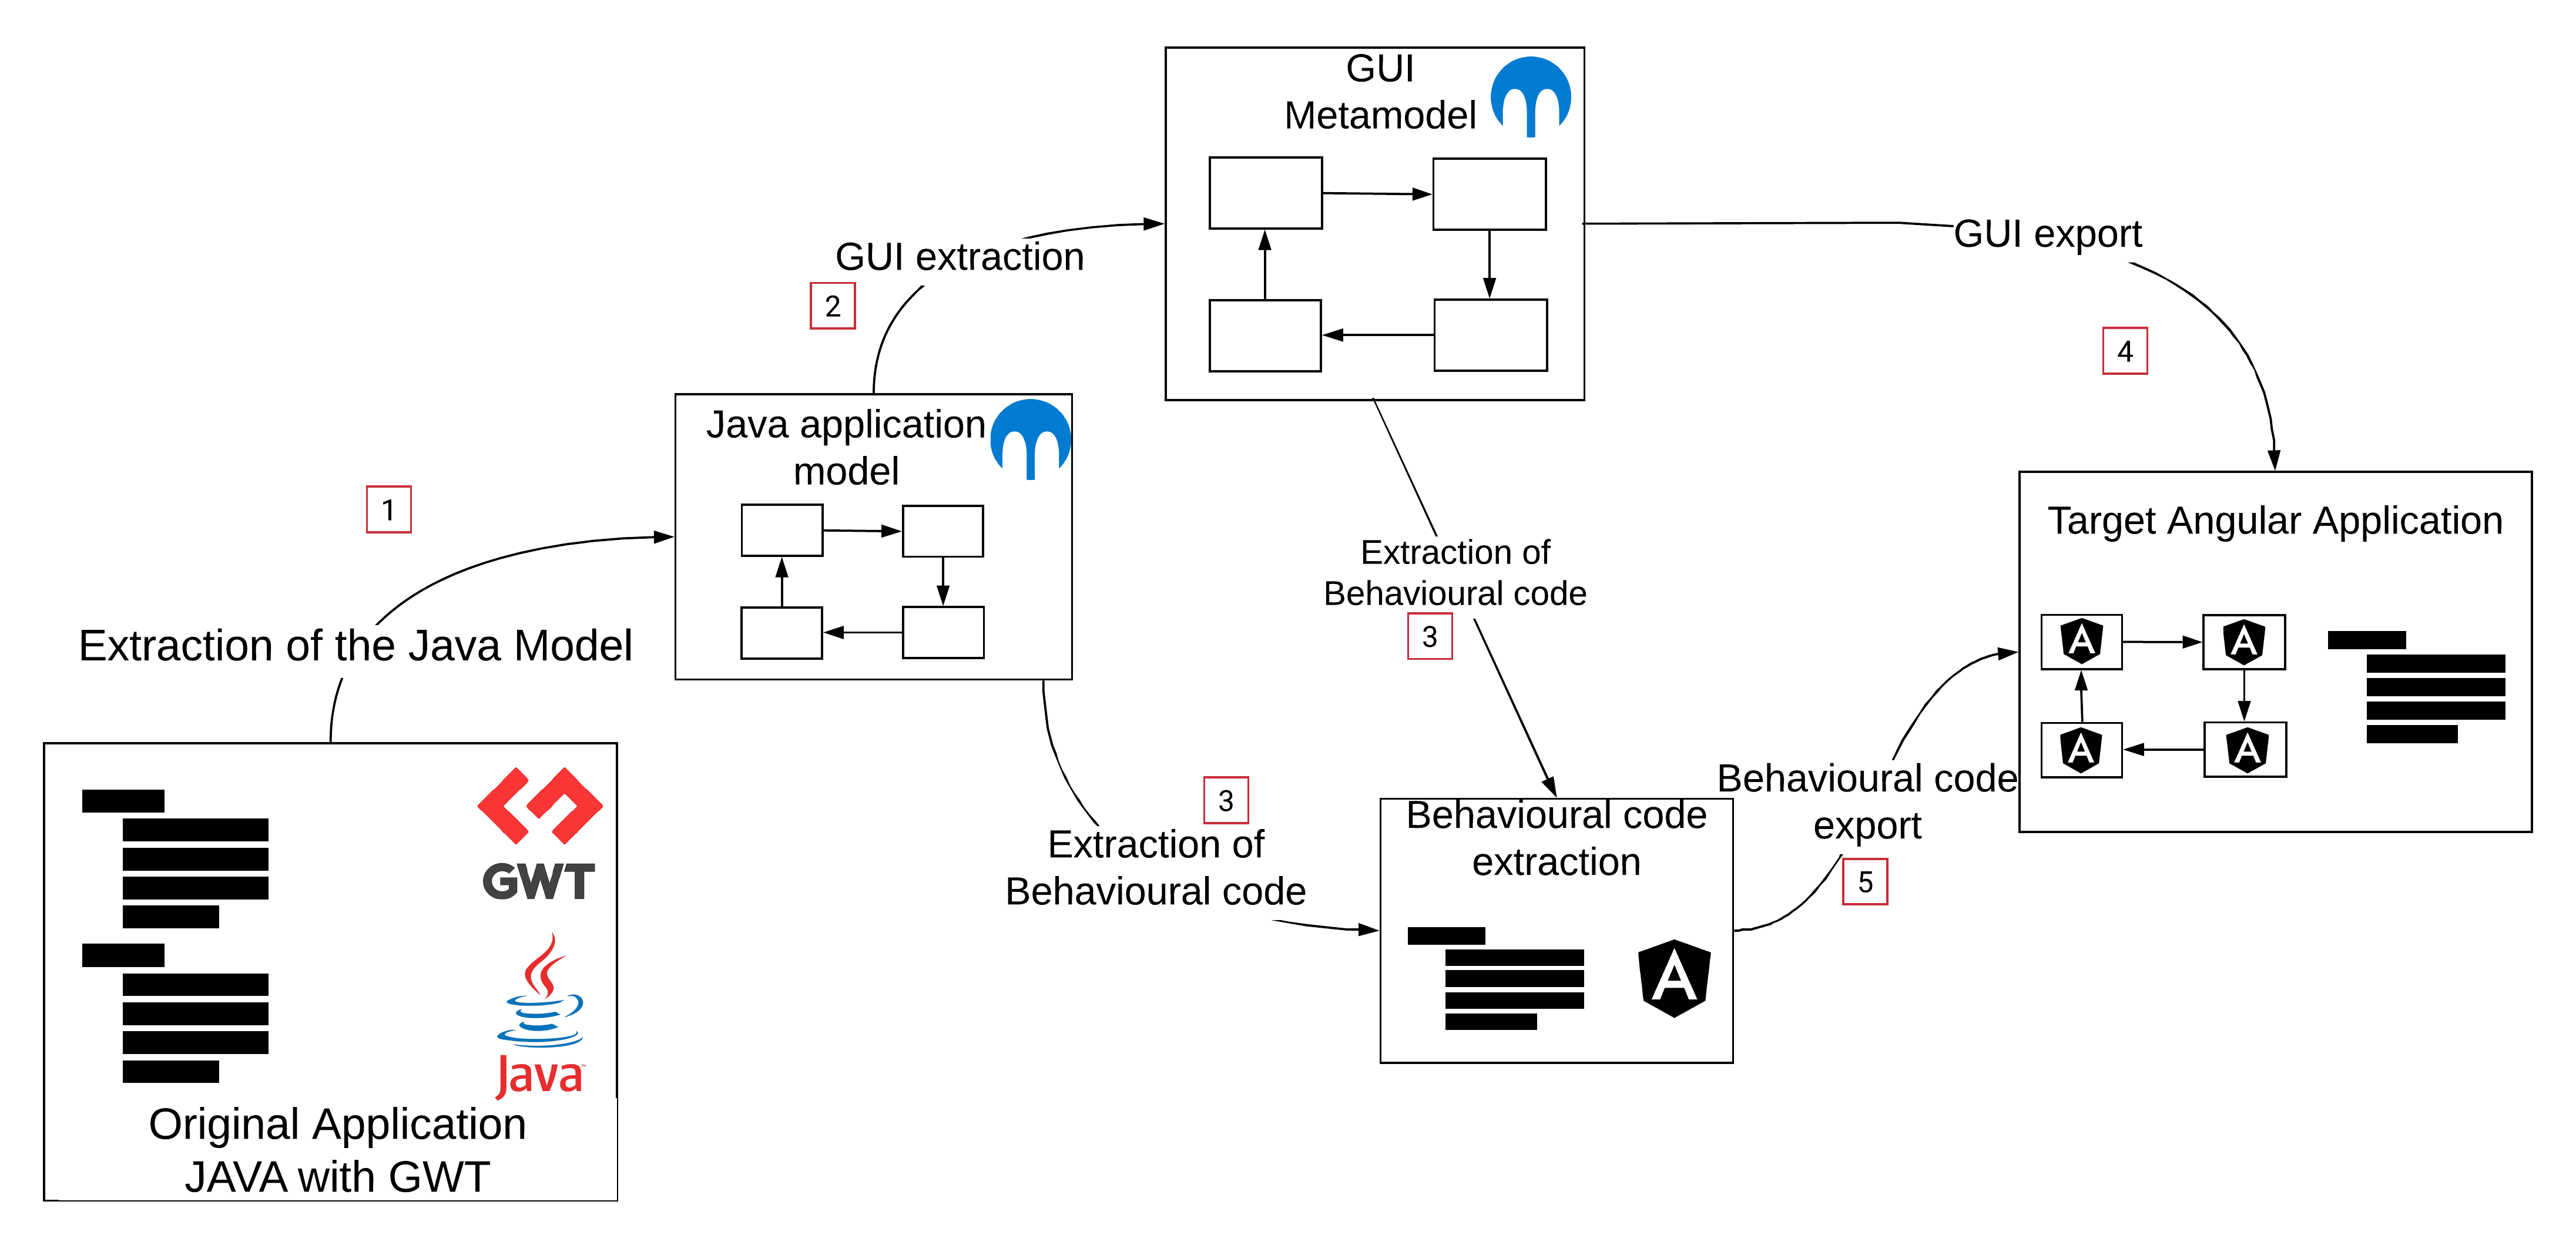
\includegraphics[width=1\textwidth,height=\textheight]{figures/processusMigration.png}
\caption{Schema processus de migration}\label{fig:processusMigration}
\end{figure}
}

À partir de l'état de l'art et des contraintes que nous avons
explicités, nous avons conçu une stratégie pour effectuer la migration.
Le processus que l'on a représenté Figure \ref{fig:processusMigration}
est divisé en cinq étapes :

\begin{enumerate}
\def\labelenumi{\arabic{enumi}.}
\tightlist
\item
  \emph{Extraction du modèle de la technologie source} est la première
  étape permettant de construire l'ensemble des analyses et
  transformations que nous devons appliquer pour effectuer la migration.
  Elle consiste en la génération d'un modèle représentant le code source
  de l'application originel. Dans notre cas d'étude, le programme source
  est en java et donc le modèle que nous créons est une implémentation
  d'un méta-modèle permettant de représenter une application écrite en
  java.
\item
  \emph{Extraction de l'interface utilisateur} est l'analyse du modèle
  de la technologie source pour détecter les éléments qui relèvent du
  modèle d'interface utilisateur. Ce dernier, que nous avons dû
  concevoir, est expliqué Section \ref{sec:metamodelUI}.
\item
  \emph{Extraction du code comportemental}. Une fois le modèle d'UI
  généré, il est possible d'extraire le code comportemental du modèle de
  la technologie source et de créer les correspondances entre les
  éléments faisant partie à la fois du code comportemental et du modèle
  d'interface utilisateur. Par exemple, si un clique sur un bouton agit
  sur un texte dans l'interface graphique. L'extraction du code
  comportemental permet de définir que pour le bouton, définit dans le
  modèle UI, lorsqu'un clique est effectué, on effectue un certain
  nombre d'actions dont une sur le texte, lui aussi définit dans le
  modèle UI.
\item
  \emph{Exportation de l'interface utilisateur}. Le modèle d'interface
  graphique étant construit et les liens entre interfaces utilisateur et
  code comportemental créés, il est possible d'effectuer l'exportation
  de l'interface utilisateur. Cela consiste à la génération du code du
  langage source exprimant uniquement l'interface graphique. C'est aussi
  à cette étape que l'on génère l'architecture des fichiers nécessaire
  au fonctionnement de l'application cible ainsi que la création des
  fichiers de configuration inhérent à l'interface.
\item
  Finalement, l'\emph{Exportation du code comportemental} est la
  génération du code comportemental qui est lié à l'interface
  utilisateur. Cette étape peut être effectuée en parallèle de la
  quatrième.
\end{enumerate}

\hypertarget{sec:metamodelUI}{%
\subsection{Méta-modèle d'interface utilisateur}\label{sec:metamodelUI}}

\hypertarget{guiModel}{%
\begin{figure}
\centering
\includegraphics[width=0.8\textwidth,height=\textheight]{figures/guiModel.png}
\caption{Méta-Modèle d'un application de
Berger-Levrault}\label{guiModel}
\end{figure}
}

Afin de représenter une interface utilisateur, nous avons conçu le
méta-model proposé Figure \ref{guiModel}. Dans la suite de cette partie,
nous présentons les différentes entités du méta-modèle.

La \textbf{Phase} représente le conteneur principal d'une page interface
utilisateur. Cela peut correspondre à une \emph{fenêtre} d'une
application du bureau, une page web, ou dans notre cas d'un onglet d'une
page web. Une Phase peut contenir plusieurs Business page. Elle peut
aussi être appelée par un widget grâce à une Call Phase Action.
Lorsqu'une Phase est appelée, l'interface change pour afficher la Phase.
Dans le cas d'une application de bureau, l'interface change ou une
nouvelle fenêtre est ouverte avec l'interface de la Phase. Avec une
application web, l'appelle d'une Phase peut correspondre à l'ouverture
d'un nouvel onglet, le changement d'onglet actif ou la transformation de
la page web courante.

Les \textbf{Widgets} sont les différents composants d'interface et les
composants de disposition. Il existe deux types de widgets. Le
\textbf{Leaf} est un widget qui ne contient pas un autre widget dans
l'interface. Le \textbf{Containers} peut contenir un autre widget. Ce
dernier permet de séparer les widgets en fonction de leur place dans
l'organisation de la page web représenté.

Les \textbf{Attributes} représentent les informations appartenant à un
Widget et peuvent changer son aspect visuel ou son comportement. Les
attributs communs sont la hauteur et la largeur pour définir précisément
la dimension d'un widget. Il y a aussi des attributs pour contenir des
attributs tels que le texte contenu par un widget. Par exemple, un
widget représentant un bouton peut avoir un attribut \emph{text}
explicite le texte du bouton. Un attribut peut changer le comportement,
ce pourrait être le cas d'un attribut \emph{enable}. Un bouton avec
l'attribut \emph{enable} positionné sur \emph{false} représente un
bouton sur lequel nous ne pouvons pas cliquer. Enfin, les widgets
peuvent avoir un attribut qui aura un impact sur le visuel de
l'application. Cet attribut définit la disposition de ses enfants et
potentiellement sa propre dimension pour respecter la mise en pages.

Les \textbf{Actions} sont propres aux Widgets. Elles représentent des
actions qui peuvent être exécutées dans une interface graphique.
\textbf{Call Service} représente un appel à un service distant tel
Internet. \textbf{Fire PopUp} est l'action qui affiche un PopUp sur
l'écran. Le PopUp ne peut pas être considéré comme un widget, il n'est
pas présent dans l'interface graphique, il apparaît seulement et
disparaît.

Le \textbf{Service} est la référence à la fonctionnalité distante que
l'application peut appeler à partir de son interface graphique. Dans un
contexte Web, il peut s'agir du côté serveur de l'application.

\hypertarget{muxe9ta-moduxe8le-du-code-comportemental}{%
\subsection{Méta-modèle du code
comportemental}\label{muxe9ta-moduxe8le-du-code-comportemental}}

\hypertarget{behavioralModel}{%
\begin{figure}
\centering
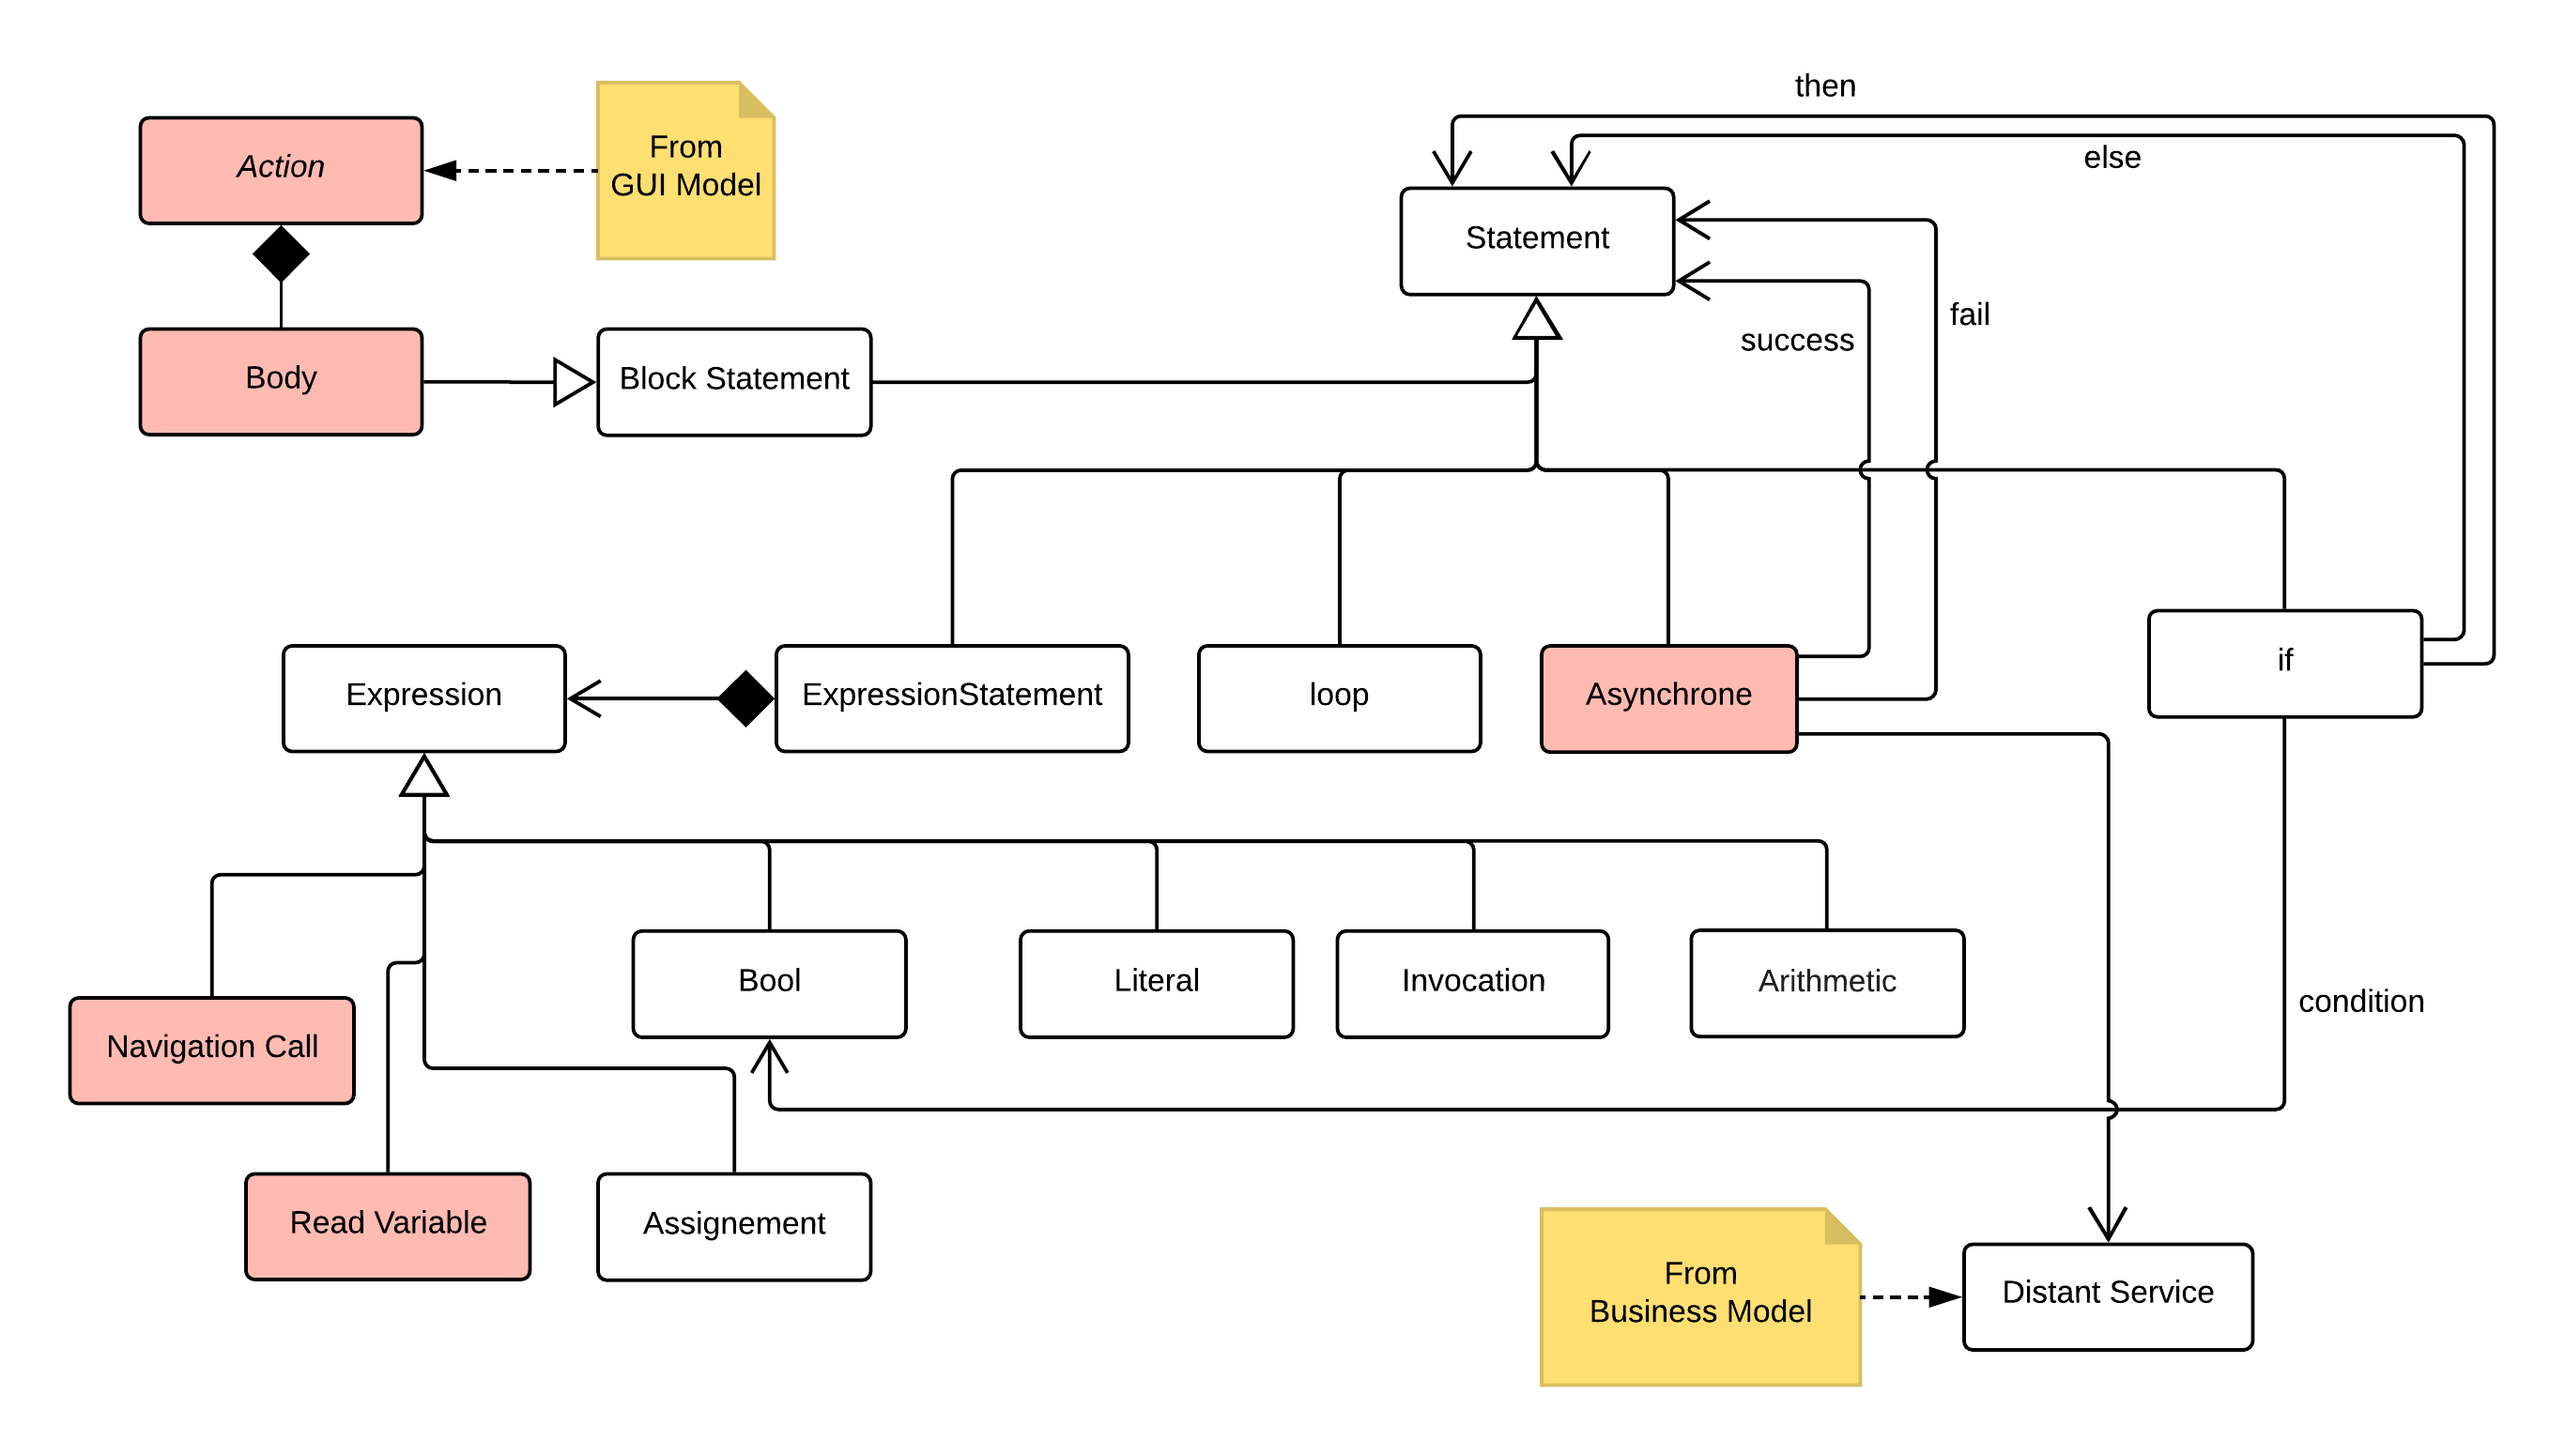
\includegraphics[width=1\textwidth,height=\textheight]{figures/behavioralModel.png}
\caption{Méta-Modèle d'un application de
Berger-Levrault}\label{behavioralModel}
\end{figure}
}

\hypertarget{impluxe9mentation-du-processus}{%
\subsection{Implémentation du
processus}\label{impluxe9mentation-du-processus}}

Pour tester la stratégie, nous avons implémenté un outil qui suit le
processus de migration. L'outil a été implémenté en Pharo\footnote{\href{http://pharo.org/}{Pharo
  est un langage de programmation objet, réflexif et dynamiquement typé
  - (http://pharo.org/)}} et nous avons utilisé la plateforme
Moose\footnote{Moose est une plateforme pour l'analyse de logiciels et
  de données - \url{http://www.moosetechnology.org/}}.

\hypertarget{codeImpl}{%
\begin{figure}
\centering
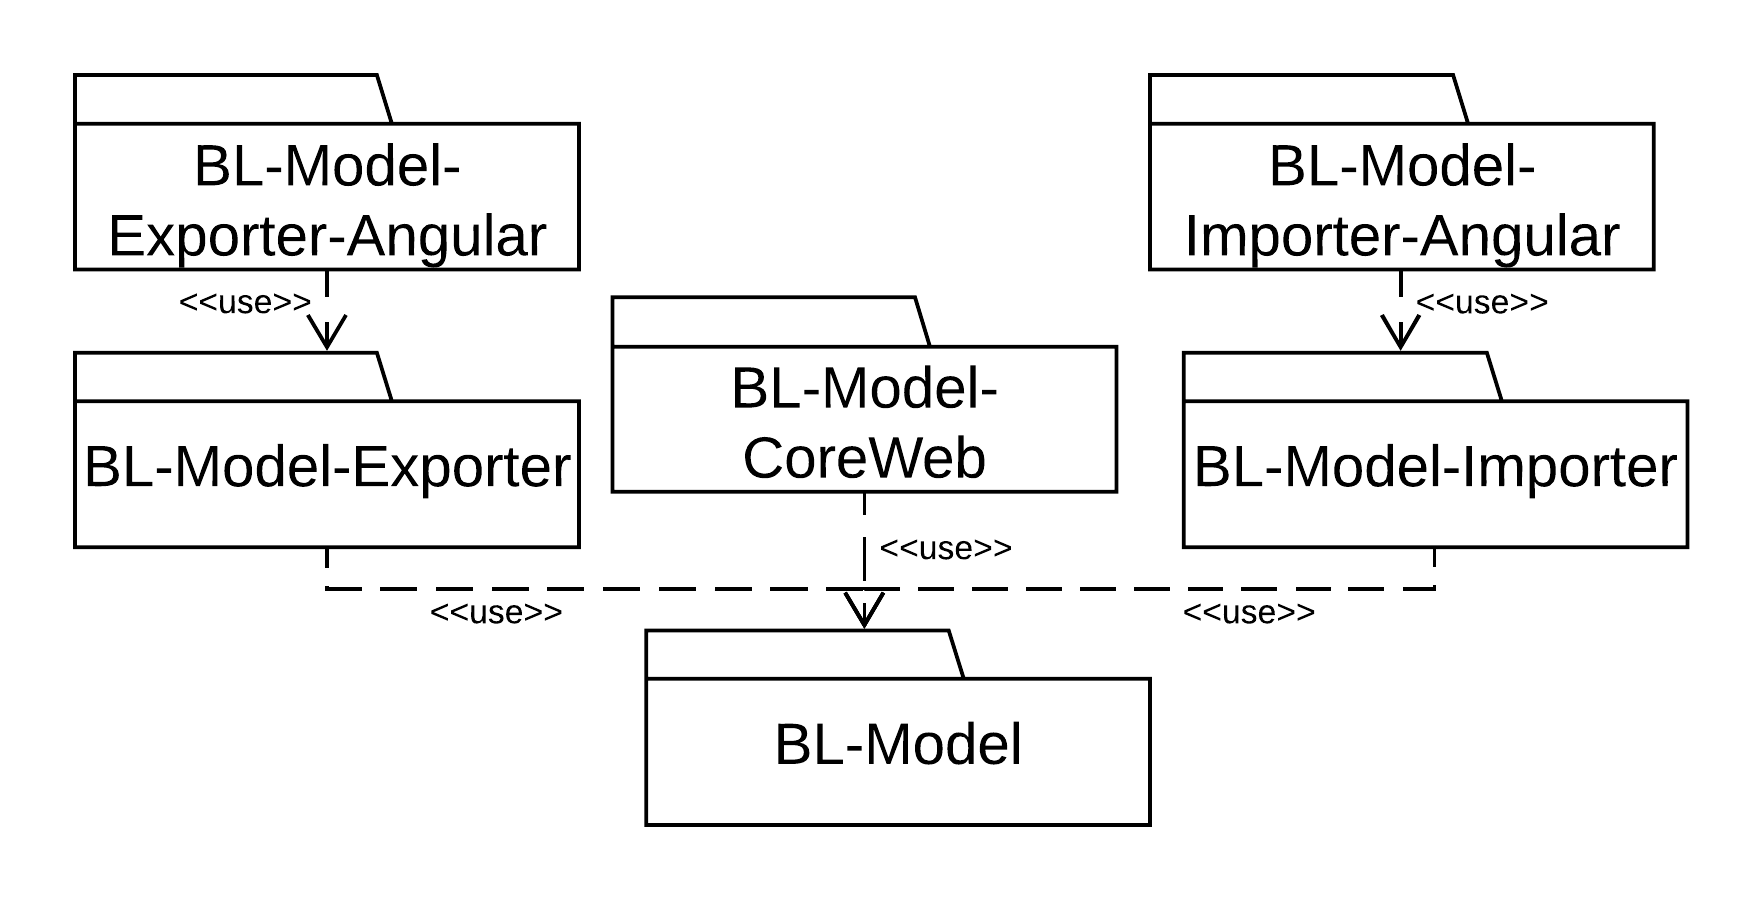
\includegraphics[width=3.64583in,height=2.60417in]{figures/codeImpl.png}
\caption{Implémentation de l'outil}\label{codeImpl}
\end{figure}
}

Le Figure \ref{codeImpl} présente la logique d'implémentation. Le bloc
principal est \emph{BL-Model}. Ce bloc contient l'implémentation du
méta-modèle GUI. En plus du modèle, il y a un exportateur abstrait et
une implémentation de l'exportateur pour Angular
(\emph{BL-Model-Exporter} et \emph{BL-Model-Exporter-Angular}, un
importateur abstrait et le code spécifique pour Java
(\emph{BL-Model-Importateur} et \emph{BL-Model-Importer-Java}). Parce
que nous testons notre solution sur le système de Berger-Levrault, nous
avons également implémenté l'extension \emph{``CoreWeb''}, alors que la
stratégie de migration ne dépend pas de cette extension. Ces paquets
étendent les précédents pour avoir un contrôle fin du processus de
migration. Ce contrôle est important pour améliorer le résultat final.

\hypertarget{meta-moduxe8le}{%
\subsubsection{Meta-modèle}\label{meta-moduxe8le}}

Pour implémenter le méta-modèle GUI (voir Figure \ref{guiModel}), nous
avons utilisé la dernière version de Famix dans Moose. Cet outil est
pratique car il fournit un générateur de méta-modèle, le builder. Pour
définir les entités du méta-modèles, il faut les nommer dans la méthode
\texttt{defineClasses} du builder. Pour les relations entre les entités,
nous pouvons utilisé le format UML. Ainsi une relation
\emph{``oneToMany''} entre deux entités se définit de la manière
suivante : \texttt{entity1\ -*\ entity2}.

Afin de tester la stratégie sur l'application de Berger-Levrault, nous
avons créé des types spécifiques de Widget pour Berger-Levrault. Des
exemple de ces widgets sont le \emph{SplitButton}, \emph{RichTextArea}
ou \emph{Switch}. Ces éléments n'appartiennent pas au modèle GUI
d'origine et, combiné avec le cadre que nous avons créé, ils rendent
l'implémentation de l'outil plus modulaire.

\hypertarget{importation}{%
\subsubsection{Importation}\label{importation}}

La création des modèles représentant l'interface graphique est divisée
en trois étapes comme présenté Section \ref{sec:processusMigration}.
Dans le cas de Berger-Levrault, nous avons implémenté la stratégie en
Pharo avec Moose.

La première étape est la conception du modèle de la technologie source.
Ce modèle avait déjà une implémentation existante dans Moose avec le
projet \emph{Famix-Java}. Nous avons donc réutilisé ce modèle pour ne
pas avoir à re-concevoir un modèle pré-existant. De plus, ce travail
préliminaire est compatible avec plusieurs outils qui ont été développés
en interne à RMod. Entre autres, deux logiciels de génération du modèle
Famix-Java depuis du code source java existait. Les outils sont
verveineJ\footnote{\href{https://rmod.inria.fr/web/software/}{verveineJ
  : https://rmod.inria.fr/web/software/}} et jdt2Famix\footnote{\href{https://github.com/feenkcom/jdt2famix}{jdt2famix
  : https://github.com/feenkcom/jdt2famix}}. Ces deux derniers
permettent de créer depuis le code source un fichier \emph{mse}. Le
fichier \emph{mse} peut ensuite être importé dans la plateforme Moose.
Pour le cas de Berger-Levrault, nous avons utilisé verveineJ car ce
dernier permet aussi de \emph{garder un lien} entre le modèle généré et
le code à partir duquel il l'a été.

Une fois le modèle de la technologie source créé, et après avoir
implémenté nos méta-modèles, nous avons développé des outils en Pharo
permettant d'effectuer la transformation du modèle source vers le modèle
GUI. Nous allons maintenant décrire les techniques utilisées pour
retrouver les éléments définis dans le modèle GUI depuis le modèle de
technologie source.

Les premiers éléments que nous avons voulu reconnaître sont les phases.
En analysant les projets GWT, nous avons repéré un fichier \emph{.xml}
dans lequel est stocké toutes les informations des phases. Nous avons
donc ajouté une étape à l'importation qui est l'analyse d'un fichier
\emph{xml}. Ce fichier nous permet de \emph{``facilement''} récupéré la
classe java correspondant à une phase, ainsi que le nom de la phase.

Ensuite, nous avons développé l'outil d'importation de manière
incrémentale. Nous avons donc cherché les Business Page. Grâce à
l'analyse préliminaire des applications de Berger-Levrault, nous avons
détecté que les business pages en GWT correspondent à des classes qui
implémente l'interface \emph{IPageMetier}. Une fois les classes
trouvées, nous avons recherché les appels des constructeurs des classes.
Puis, en faisant le lien entre le constructeur et la phase qui
\emph{``ajoute''} la business page à leur contenu, nous avons détecté
les liens d'appartenances entre les pages métiers et les phases.

Pour les widgets, nous avons dû tout d'abord trouver tous les widgets
potentiellement instanciable. Pour cela, nous avons cherché toutes les
sous-classes java de la classe GWT \emph{Widget}. Ce sont les classes
qui vont pouvoir être instancié et utilisé pour la construction du
programme. Ensuite, comme pour les business pages, nous avons cherché
les appels des constructeurs des widgets et avons relié ces appels à la
business page qui les a ajouté.

Enfin, pour la détection des attributs et des actions associés à un
widget. Nous avons, pour chaque widget, cherché dans quelle variable
java il a été affecté. Puis nous avons cherché les appels de méthodes
effectué depuis ces variables java. Les appels aux méthodes
\emph{``addActionHandler''} sont transformés en action tandis que les
appels aux méthodes \emph{``setX''} ont été transformé en attribut.

\hypertarget{exportation}{%
\subsubsection{Exportation}\label{exportation}}

Une fois la génération du modèle d'interface graphique et du modèle du
code comportemental terminé, il est possible de lancer l'exportation.
L'exportation consiste en la génération du code source de l'application
cible.

La première étape de l'implémentation de l'exportation est l'utilisation
d'un patron de conception \emph{``visiteur''}. Ce dernier est ajouté au
modèle d'interface graphique, aux phases et business pages.

La visite du modèle GUI va créer la hiérarchie de l'application cible
ainsi que les fichiers de configuration. Ensuite, l'exportation visite
toutes les phases. Pour chacune des phases, considéré comme des
sous-projets en Angular dans l'architecture de l'application cible que
nous avons défini, le visiteur génère les fichiers de configurations.
Puis, pour chaque business page, le visiteur va générer un fichier HTML
et un fichier TypeScript. Pour le fichier html, le visiteur construit le
DOM à partir des widgets contenu dans la business page. Les widgets
connaissant leurs attributs et actions, ils fournissent eux-mêmes leurs
caractéristiques aux visiteurs. Ces caractéristiques englobent la
génération du code comportemental.

\newpage

\hypertarget{ruxe9sultats-et-discussion}{%
\section{Résultats et Discussion}\label{ruxe9sultats-et-discussion}}

Nous allons maintenant présenter les résultats que nous avons obtenus
suite à l'implémentation de la stratégies de migration.

\hypertarget{ruxe9sultats}{%
\subsection{Résultats}\label{ruxe9sultats}}

\hypertarget{visualisation}{%
\subsection{Visualisation}\label{visualisation}}

\hypertarget{firework}{%
\begin{figure}
\centering
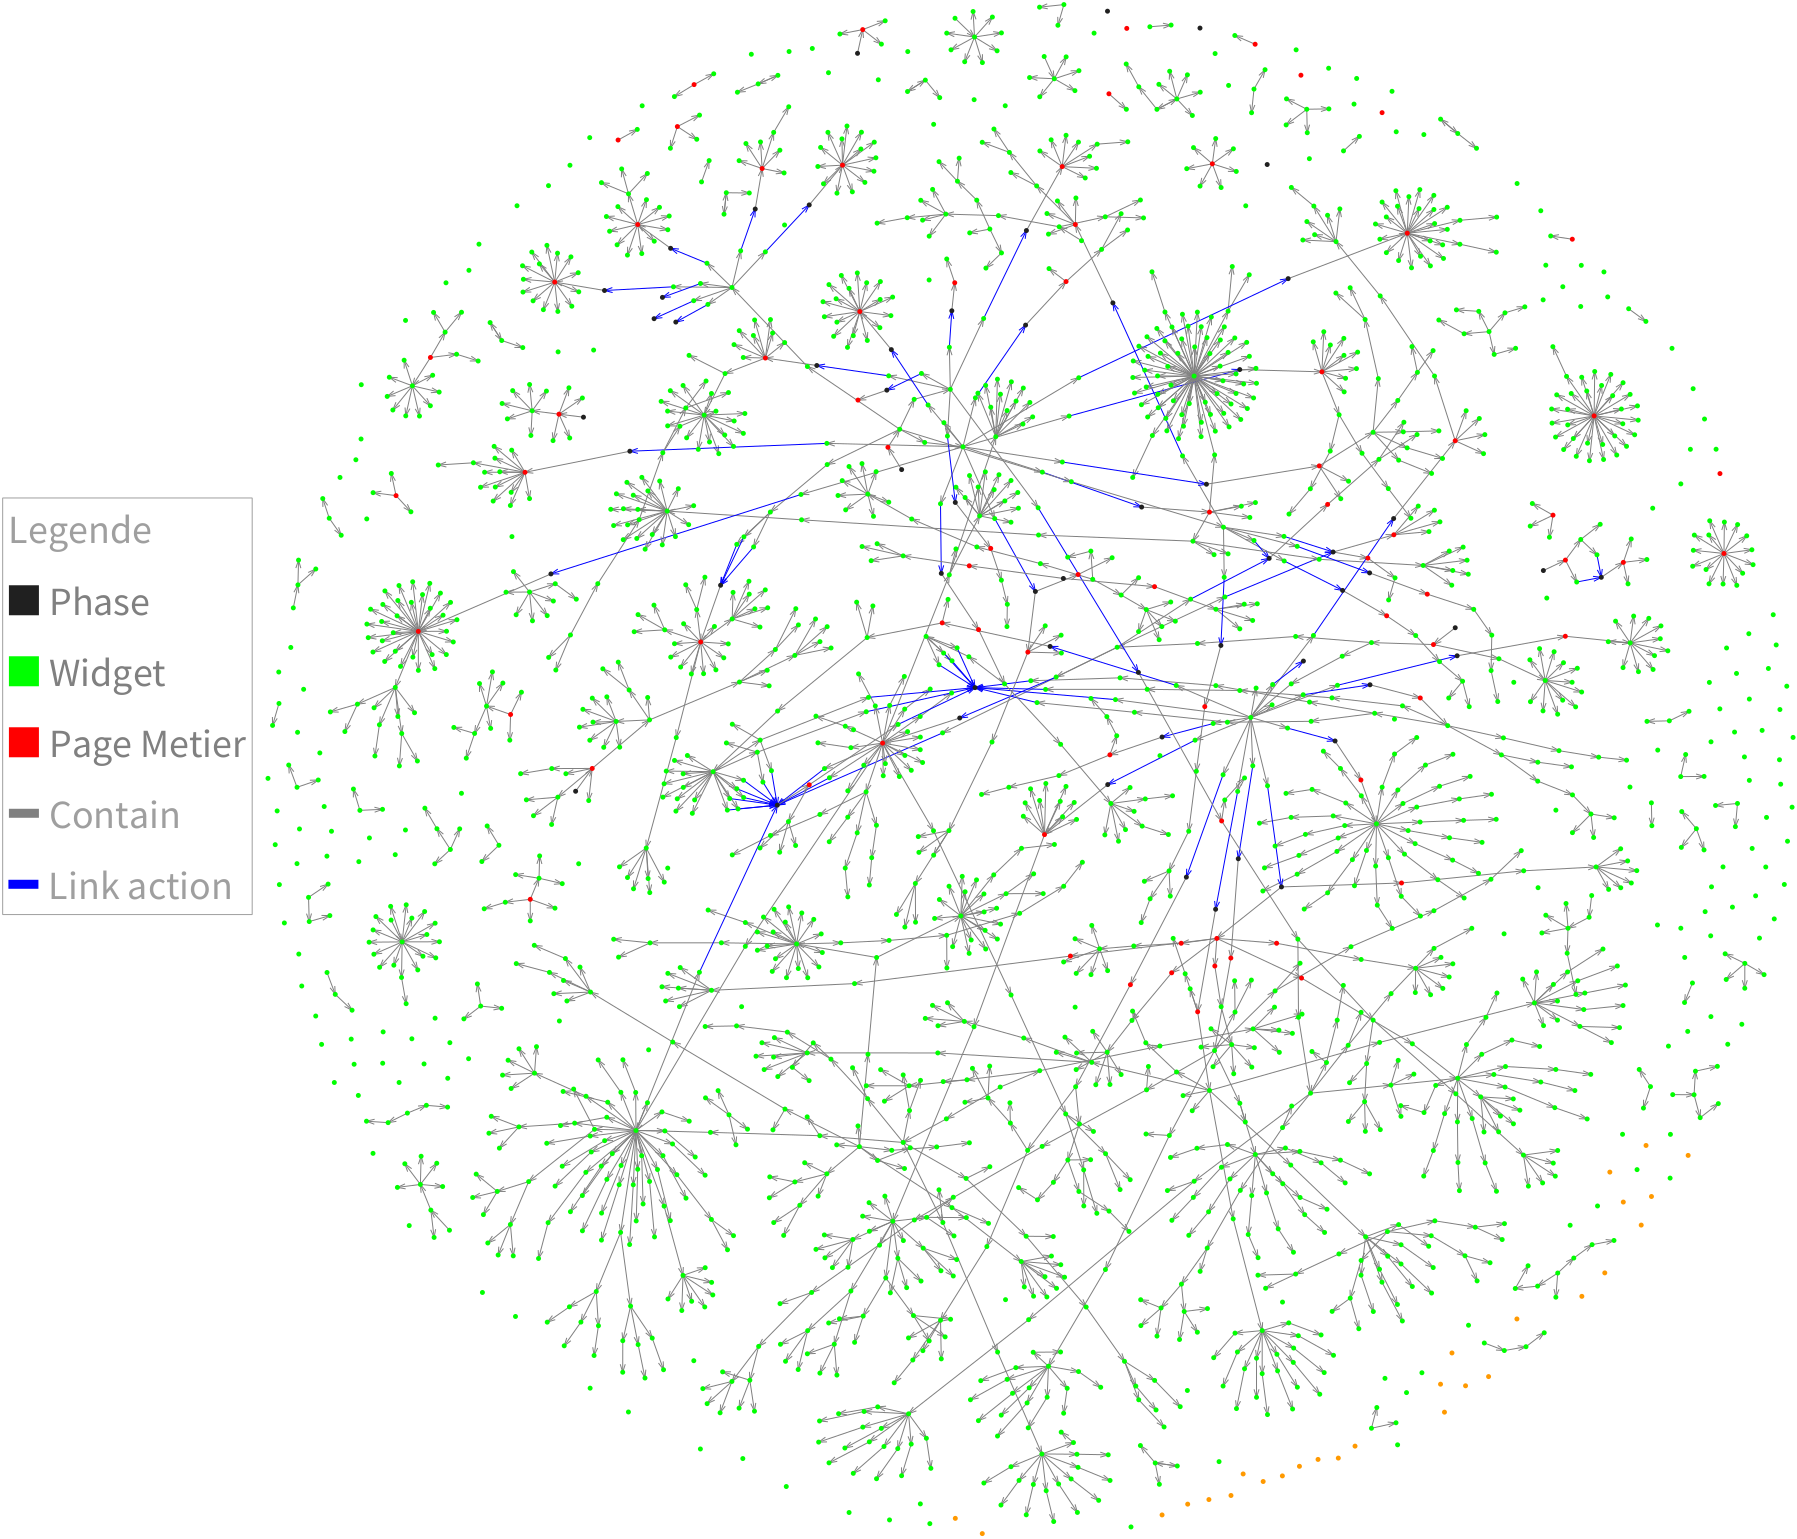
\includegraphics[width=1\textwidth,height=\textheight]{figures/firework.png}
\caption{Représentation de l'application bac à sable dans sa
globalité}\label{firework}
\end{figure}
}

\hypertarget{discussion}{%
\subsection{Discussion}\label{discussion}}

\begin{itemize}
\tightlist
\item
  Les évaluation n'ont été faîte que sur l'application
  \emph{bac-à-sable}
\item
  Il n'y a pas de gestion de certaine manière de décrire une interface
  en GWT (cf xml file) - mais ça ne sera pas fait
\item
  La migration de l'application ici ne prend pas en compte les
  éventuelles evolutions parallèle du backend
\end{itemize}

\newpage

\hypertarget{travaux-futurs}{%
\section{Travaux futurs}\label{travaux-futurs}}

Il manque

\begin{itemize}
\tightlist
\item
  layout
\item
  behavior complet
\item
  outil de validation
\item
  business code
\item
  missing widget
\end{itemize}

\newpage

\hypertarget{conclusion}{%
\section{Conclusion}\label{conclusion}}

Durant ce stage, j'ai continué le projet de migration que j'ai initié
pendant mon projet de fin d'études à Polytech Lille. Après une première
étape d'analyse que j'avais menée durant ce stage, j'ai approfondi les
recherches de l'état de l'art et créer des outils permettant de
faciliter la migration des applications de Berger-Levrault.

La première étape de mon stage a été la définition formelle des éléments
composant une application d'une interface graphique. Une application
graphique est divisée en trois parties, l'interface graphique, le code
comportemental et le code métier. Ensuite, j'ai défini les différentes
contraintes à respecter pour répondre aux besoins de Berger-Levrault et
conçu un processus permettant d'effectuer la migration en suivant ces
obligations. Puis, j'ai implémenté en partie les outils nécessaires pour
effectuer la migration en suivant le processus de migration. Ainsi, j'ai
pu commencer l'exportation de certains éléments des applications GWT en
Angular.

La stratégie de migration est bien définie et que l'implémentation du
modèle d'interface graphique avec les outils d'importation et
d'exportation donnent des résultats encourageant sur la suite du projet.
Il reste encore du travail d'implémentation et de définition de
méta-modèles. En effet, je n'ai pas encore conçu les méta-modèles pour
les \emph{layout}, le code comportemental et le code métier. Une fois
conçus, il faudra les implémenter tout en gardant la structure du projet
cohérent.

Un autre travail doit être mené sur la validation des résultats. En
effet, même si pour les cas simples que nous avons étudié il est
possible de vérifier la validé de l'exportation \emph{``à la main''},
une fois l'exportation complètement implémentée, il faudra développer
des outils permettant d'évaluer la complétude de mon travail. \newpage

\hypertarget{bibliographie}{%
\section*{Bibliographie}\label{bibliographie}}
\addcontentsline{toc}{section}{Bibliographie}

\hypertarget{refs}{}
\leavevmode\hypertarget{ref-samir2007swing2script}{}%
{[}1{]} H. Samir, E. Stroulia, and A. Kamel, ``Swing2script: Migration
of java-swing applications to ajax web applications,'' in \emph{Reverse
engineering, 2007. WCRE 2007. 14th working conference on}, 2007, pp.
179--188.

\leavevmode\hypertarget{ref-staiger2007reverse}{}%
{[}2{]} S. Staiger, ``Reverse engineering of graphical user interfaces
using static analyses,'' in \emph{Reverse engineering, 2007. WCRE 2007.
14th working conference on}, 2007, pp. 189--198.

\leavevmode\hypertarget{ref-morgado2011reverse}{}%
{[}3{]} I. C. Morgado, A. Paiva, and J. P. Faria, ``Reverse engineering
of graphical user interfaces,'' in \emph{The sixth international
conference on software engineering advances, barcelona}, 2011, pp.
293--298.

\leavevmode\hypertarget{ref-shah2011reverse}{}%
{[}4{]} E. Shah and E. Tilevich, ``Reverse-engineering user interfaces
to facilitateporting to and across mobile devices and platforms,'' in
\emph{Proceedings of the compilation of the co-located workshops on
dsm'11, tmc'11, agere! 2011, aoopes'11, neat'11, \& vmil'11}, 2011, pp.
255--260.

\leavevmode\hypertarget{ref-sanchez2014model}{}%
{[}5{]} Ó. Sánchez Ramón, J. Sánchez Cuadrado, and J. García Molina,
``Model-driven reverse engineering of legacy graphical user
interfaces,'' in \emph{Proceedings of the ieee/acm international
conference on automated software engineering}, 2014, pp. 147--186.

\leavevmode\hypertarget{ref-silva2010guisurfer}{}%
{[}6{]} J. C. Silva, C. Silva, R. D. Gonçalo, J. Saraiva, and J. C.
Campos, ``The guisurfer tool: Towards a language independent approach to
reverse engineering gui code,'' in \emph{Proceedings of the 2nd acm
sigchi symposium on engineering interactive computing systems}, 2010,
pp. 181--186.

\leavevmode\hypertarget{ref-gotti2016java}{}%
{[}7{]} Z. Gotti and S. Mbarki, ``Java swing modernization approach:
Complete abstract representation based on static and dynamic analysis,''
in \emph{ICSOFT-ea}, 2016, pp. 210--219.

\leavevmode\hypertarget{ref-MemonWCRE2003}{}%
{[}8{]} A. M. Memon, I. Banerjee, and A. Nagarajan, ``GUI ripping:
Reverse engineering of graphical user interfaces for testing,'' in
\emph{Proceedings of the 10th working conference on reverse
engineering}, 2003.

\leavevmode\hypertarget{ref-lelli2016automatic}{}%
{[}9{]} V. Lelli, A. Blouin, B. Baudry, F. Coulon, and O. Beaudoux,
``Automatic detection of gui design smells: The case of blob listener,''
in \emph{Proceedings of the 8th acm sigchi symposium on engineering
interactive computing systems}, 2016, pp. 263--274.

\leavevmode\hypertarget{ref-cloutier2016wavi}{}%
{[}10{]} J. Cloutier, S. Kpodjedo, and G. El Boussaidi, ``WAVI: A
reverse engineering tool for web applications,'' 2016, pp. 1--3.

\leavevmode\hypertarget{ref-aho2013industrial}{}%
{[}11{]} P. Aho, M. Suarez, T. Kanstrén, and A. M. Memon, ``Industrial
adoption of automatically extracted gui models for testing.'' in
\emph{EESSMOD models}, 2013, pp. 49--54.

\leavevmode\hypertarget{ref-teyton2013automatic}{}%
{[}12{]} C. Teyton, J.-R. Falleri, and X. Blanc, ``Automatic discovery
of function mappings between similar libraries,'' in \emph{Reverse
engineering (wcre), 2013 20th working conference on}, 2013, pp.
192--201.

\leavevmode\hypertarget{ref-hora2015automatic}{}%
{[}13{]} A. Hora, N. Anquetil, A. Etien, S. Ducasse, and M. T. Valente,
``Automatic detection of system-specific conventions unknown to
developers,'' \emph{Journal of Systems and Software}, vol. 109, pp.
192--204, 2015.

\leavevmode\hypertarget{ref-zhong2010mining}{}%
{[}14{]} H. Zhong, S. Thummalapenta, T. Xie, L. Zhang, and Q. Wang,
``Mining api mapping for language migration,'' in \emph{Proceedings of
the 32nd acm/ieee international conference on software
engineering-volume 1}, 2010, pp. 195--204.

\leavevmode\hypertarget{ref-nguyen2014statistical}{}%
{[}15{]} A. T. Nguyen, H. A. Nguyen, T. T. Nguyen, and T. N. Nguyen,
``Statistical learning approach for mining api usage mappings for code
migration,'' in \emph{Proceedings of the 29th acm/ieee international
conference on automated software engineering}, 2014, pp. 457--468.

\leavevmode\hypertarget{ref-phan2017statistical}{}%
{[}16{]} H. D. Phan, A. T. Nguyen, T. D. Nguyen, and T. N. Nguyen,
``Statistical migration of api usages,'' in \emph{Software engineering
companion (icse-c), 2017 ieee/acm 39th international conference on},
2017, pp. 47--50.

\leavevmode\hypertarget{ref-chen2016mining}{}%
{[}17{]} C. Chen, S. Gao, and Z. Xing, ``Mining analogical libraries in
q\&a discussions--incorporating relational and categorical knowledge
into word embedding,'' in \emph{Software analysis, evolution, and
reengineering (saner), 2016 ieee 23rd international conference on},
2016, vol. 1, pp. 338--348.

\leavevmode\hypertarget{ref-baki2016multi}{}%
{[}18{]} I. Baki and H. Sahraoui, ``Multi-step learning and adaptive
search for learning complex model transformations from examples,''
\emph{ACM Transactions on Software Engineering and Methodology (TOSEM)},
vol. 25, no. 3, p. 20, 2016.

\leavevmode\hypertarget{ref-falleri2008metamodel}{}%
{[}19{]} J.-R. Falleri, M. Huchard, M. Lafourcade, and C. Nebut,
``Metamodel matching for automatic model transformation generation,'' in
\emph{International conference on model driven engineering languages and
systems}, 2008, pp. 326--340.

\leavevmode\hypertarget{ref-wang2017automatic}{}%
{[}20{]} T. Wang, S. Truptil, and F. Benaben, ``An automatic
model-to-model mapping and transformation methodology to serve
model-based systems engineering,'' \emph{Information Systems and
e-Business Management}, vol. 15, no. 2, pp. 323--376, 2017.

\leavevmode\hypertarget{ref-fleurey2007model}{}%
{[}21{]} F. Fleurey, E. Breton, B. Baudry, A. Nicolas, and J.-M.
Jézéquel, ``Model-driven engineering for software migration in a large
industrial context,'' in \emph{International conference on model driven
engineering languages and systems}, 2007, pp. 482--497.

\leavevmode\hypertarget{ref-garces2017white}{}%
{[}22{]} K. Garcés \emph{et al.}, ``White-box modernization of legacy
applications: The oracle forms case study,'' \emph{Computer Standards \&
Interfaces}, 2017.

\leavevmode\hypertarget{ref-mukherjee2011automatic}{}%
{[}23{]} S. Mukherjee and T. Chakrabarti, ``Automatic algorithm
specification to source code translation,'' \emph{Indian Journal of
Computer Science and Engineering (IJCSE)}, vol. 2, no. 2, pp. 146--159,
2011.

\leavevmode\hypertarget{ref-brant2010extreme}{}%
{[}24{]} J. Brant, D. Roberts, B. Plendl, and J. Prince, ``Extreme
maintenance: Transforming delphi into c,'' in \emph{Software maintenance
(icsm), 2010 ieee international conference on}, 2010, pp. 1--8.

\leavevmode\hypertarget{ref-newman2017simplifying}{}%
{[}25{]} C. D. Newman, B. Bartman, M. L. Collard, and J. I. Maletic,
``Simplifying the construction of source code transformations via
automatic syntactic restructurings,'' \emph{Journal of Software:
Evolution and Process}, vol. 29, no. 4, 2017.

\leavevmode\hypertarget{ref-rolim2017learning}{}%
{[}26{]} R. Rolim \emph{et al.}, ``Learning syntactic program
transformations from examples,'' in \emph{Proceedings of the 39th
international conference on software engineering}, 2017, pp. 404--415.

\leavevmode\hypertarget{ref-feldman1990fortran}{}%
{[}27{]} S. I. Feldman, ``A fortran to c converter,'' in \emph{ACM
sigplan fortran forum}, 1990, vol. 9, pp. 21--22.

\leavevmode\hypertarget{ref-grosse2012automatic}{}%
{[}28{]} R. W. Grosse-Kunstleve, T. C. Terwilliger, N. K. Sauter, and P.
D. Adams, ``Automatic fortran to c++ conversion with fable,''
\emph{Source code for biology and medicine}, vol. 7, no. 1, p. 5, 2012.

\newpage

\hypertarget{annexe}{%
\section{Annexe}\label{annexe}}

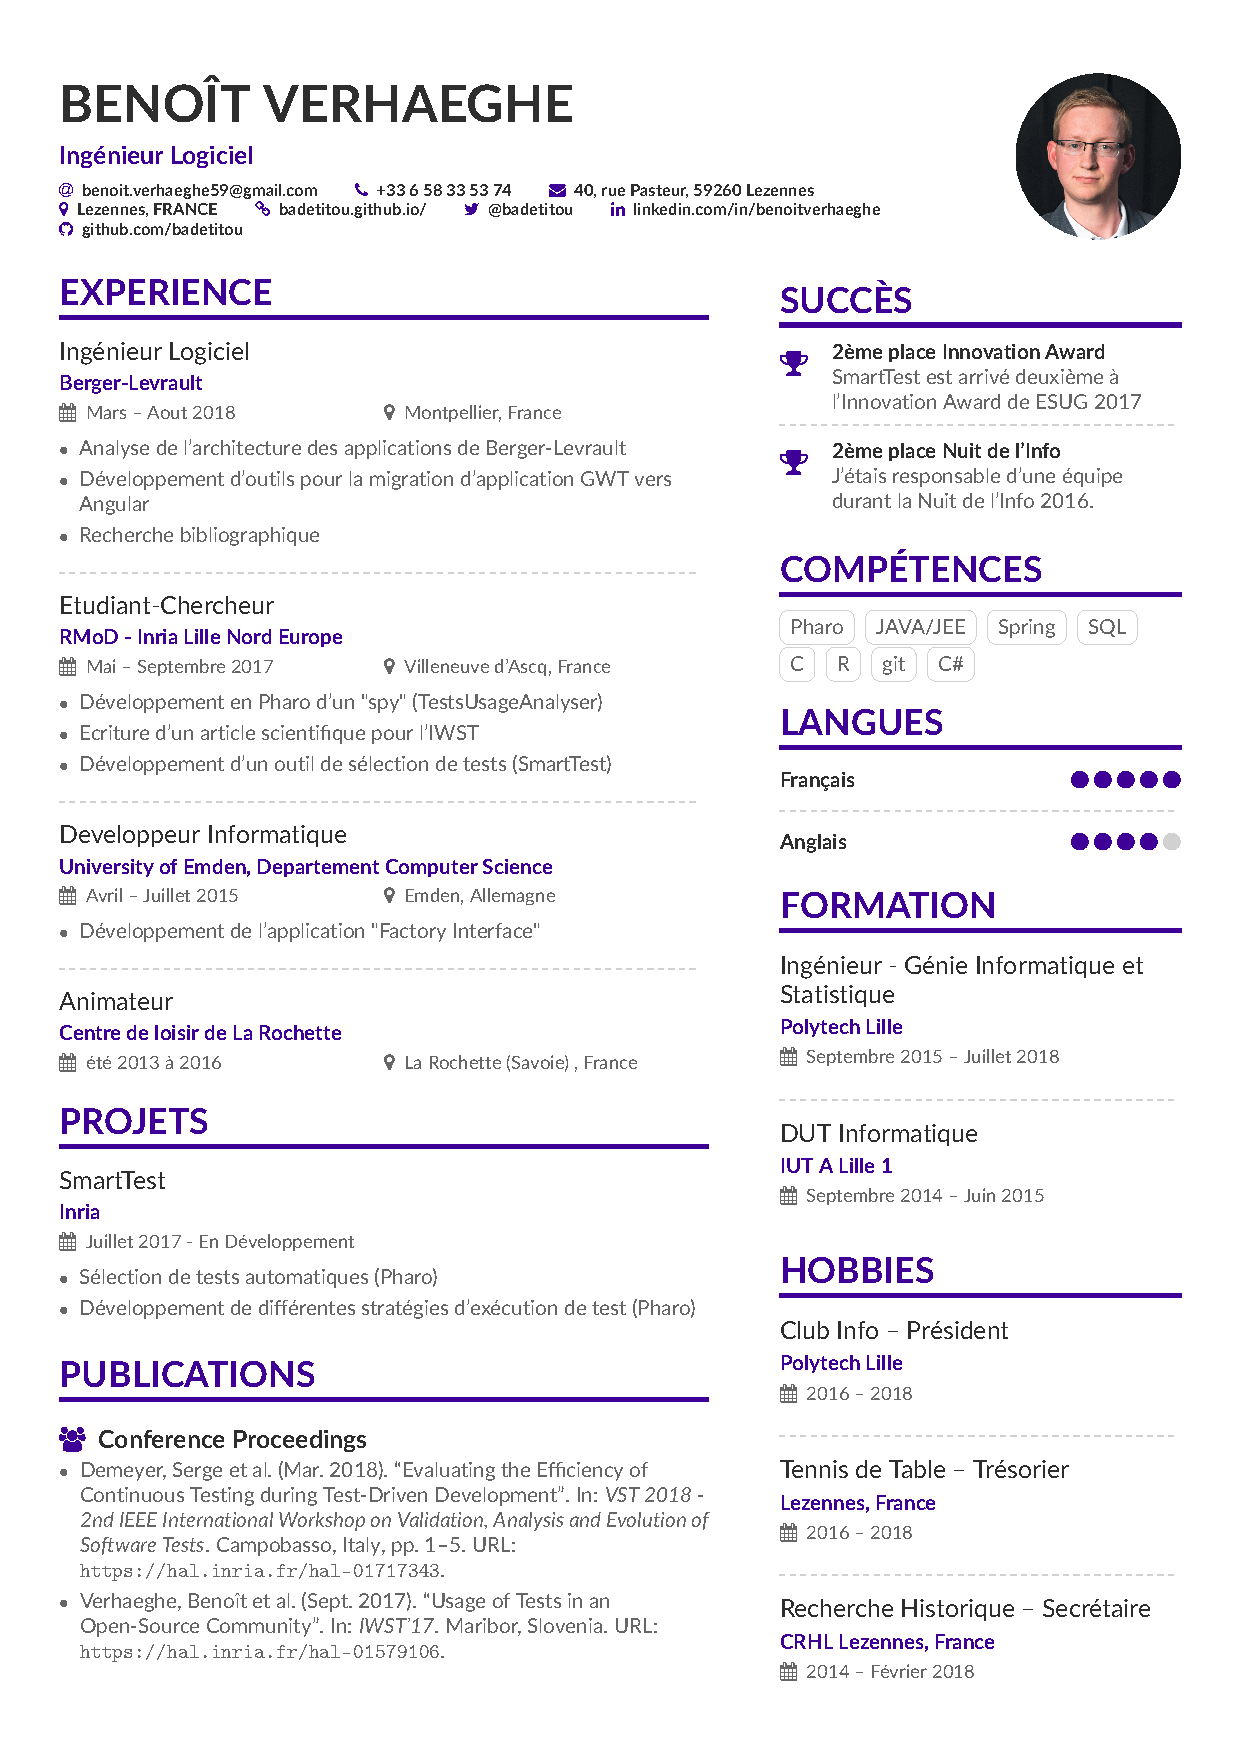
\includegraphics[width=0.9\textwidth,height=\textheight]{cv/cv.pdf}
\newpage

\hypertarget{ruxe9sumuxe9}{%
\section*{Résumé}\label{ruxe9sumuxe9}}
\addcontentsline{toc}{section}{Résumé}

\hypertarget{franuxe7ais}{%
\subsection*{Français}\label{franuxe7ais}}
\addcontentsline{toc}{subsection}{Français}

\hypertarget{anglais}{%
\subsection*{Anglais}\label{anglais}}
\addcontentsline{toc}{subsection}{Anglais}

\end{document}
